
%% bare_jrnl.tex
%% V1.4b
%% 2015/08/26
%% by Michael Shell
%% see http://www.michaelshell.org/
%% for current contact information.
%%
%% This is a skeleton file demonstrating the use of IEEEtran.cls
%% (requires IEEEtran.cls version 1.8b or later) with an IEEE
%% journal paper.
%%
%% Support sites:
%% http://www.michaelshell.org/tex/ieeetran/
%% http://www.ctan.org/pkg/ieeetran
%% and
%% http://www.ieee.org/

\documentclass[journal]{IEEEtran}

% *** PACKAGES ***
\usepackage{algorithm, algorithmic}
\usepackage{amsmath}
\usepackage{amssymb}
\usepackage{amsthm}
\newtheorem{assumption}{Assumption}
\usepackage{booktabs}
\usepackage[noadjust]{cite}
\usepackage{caption}
\usepackage{color}
\usepackage{enumerate}
\usepackage{longtable}
\usepackage{mathtools}
\usepackage{multirow}
\usepackage{url}
\usepackage[caption=false, ...]{subfig}

\newcommand{\mysection}{Section}
\newcommand{\mytitle}{section}
\newcommand{\myabrv}{sec:}
\newcommand{\mysubsection}[1]{\subsection{#1}}
\newcommand{\mysubsubsection}[1]{\subsubsection{#1}}


% *** GRAPHICS RELATED PACKAGES ***
%
\ifCLASSINFOpdf
\usepackage[pdftex]{graphicx}
  % declare the path(s) where your graphic files are
 \graphicspath{{../Figures/}}
  % and their extensions so you won't have to specify these with
  % every instance of \includegraphics
  \DeclareGraphicsExtensions{.pdf,.jpeg,.png}
  \else
  % or other class option (dvipsone, dvipdf, if not using dvips). graphicx
  % will default to the driver specified in the system graphics.cfg if no
  % driver is specified.
  % \usepackage[dvips]{graphicx}
  % declare the path(s) where your graphic files are
  % \graphicspath{{../eps/}}
  % and their extensions so you won't have to specify these with
  % every instance of \includegraphics
  % \DeclareGraphicsExtensions{.eps}
\fi

% correct bad hyphenation here
%\hyphenation{op-tical net-works semi-conduc-tor}

\newtheoremstyle{break}%
{}{}%
{\itshape}{}%
{\bfseries}{}% % Note that final punctuation is omitted.
{\newline}{}

\makeatletter
\newcommand{\removelatexerror}{\let\@latex@error\@gobble}
\makeatother

\begin{document}
% Do not put math or special symbols in the title.
\title{Multi-Target Tracking\\ via Mixed Integer Optimization}


% author names and IEEE memberships
\author{Dimitris~Bertsimas,~Zachary~Saunders, and Shimrit~Shtern}

% make the title area
\maketitle

% As a general rule, do not put math, special symbols or citations
% in the abstract or keywords.
\begin{abstract}
The field of multi-target tracking (MTT) faces two primary challenges: (i) data association and (ii) trajectory estimation. Many algorithms, such as the MHT and JPDAF, attempt to solve the MTT problem via probabilistic approaches, while few employ the use of optimization models. In this paper we take a new approach to the MTT problem by modeling it as a mixed integer optimization (MIO) model, making no probabilistic assumptions on the data. We model the basic case where there is no detection ambiguity, \textit{i.e.}, no false alarms or missed detections, and extend it to the more difficult robust case where there exists detection ambiguity. These models solve the data association and trajectory estimation problems simultaneously by minimizing an easily interpretable global objective function. Additionally, we propose a greedy heuristic that scales efficiently and finds high quality solutions in milliseconds, and we show that these heuristic solutions can be used effectively as a warm start for the MIO, enabling the MIO to achieve good solutions in seconds. In the basic case, the model has no tunable parameters and the extension to the ambiguous case requires only two easily understood parameters which serve as objective function penalties. Furthermore, we introduce a new metric for measuring complexity in the data association problem as well as a metric for measuring the performance of trajectory estimation. Numerical results show that in the case of the basic model we obtain a good reconstruction of the original tracks for a range of scenarios, while in the robust case, for small to medium sized scenarios we are able to both estimate the correct number of targets as well as correctly reconstruct the trajectories.
\end{abstract}

% Note that keywords are not normally used for peer review papers.
\begin{IEEEkeywords}
data association; mixed integer optimization; multi-target tracking; optimization; trajectory estimation
\end{IEEEkeywords}

\section{Introduction}\label{sec: Intro}
Multi-target tracking is the problem of estimation the state of multiple dynamic objects, referred to as \textit{targets} over a fixed window of time. At various points of time within the window, the targets are observed in a \textit{scan}, resulting in set of \textit{detections}. From these detections, the multi-target tracking problem aims to extract information about target dynamics. 

Solutions to this problem are sought across many civilian and military applications including but not limited to ballistic missile and aircraft defense, space applications, the movement of ships and ground troops, autonomous vehicles and robotics, and air traffic control. Each application has unique attributes and assumptions, and various algorithms have been developed for each. As a result, the field of multi-target tracking has expanded to numerous research venues, and there is a wide range of literature on the topic. A complete overview of all MTT methods, including the classes of algorithms and their variants as well as additional methods not discussed in this paper, can be found in \cite{MTT-Taxonomy}. For a more exhaustive overview of estimation techniques, filtering, gating, and more please see \cite{Bar-Shalom_MTT} and \cite{Bar-Shalom_Estimation}.

The field of multi-target tracking faces two primary challenges: (i) data association and (ii) trajectory estimation.  Given a set of sensor detections, the data association problem consists of assigning the detections to a set of targets. Alternatively, this can be viewed as a labeling problem in which each detection needs to be labeled with a target identifier. The association problem is further complicated when sensors fail to report detections (missed detection) or incorrectly report detections (false alarm), resulting in ambiguity in the number of existing targets. The trajectory estimation problem consists of estimating the state space of a target (\textit{i.e.}, position, velocity, acceleration, size, etc.) from the associated detections of the aforementioned assignment problem. Even when all of the associations are known, the estimation problem is challenging due to the presence of measurement noise. As can be seen, the two problems of data association and trajectory estimation are closely related and dependent on one another. 

Some classical algorithms treat the data association and trajectory estimation problems separately using a combination of probabilistic approaches to determine data associations and filters to estimate trajectories. One such algorithm is the global nearest neighbor (GNN). The GNN algorithm is a naive 2-D assignment algorithm, which evaluates one scan of detections at a time, globally assigning the nearest detection at each scan \cite{GNN}. Once the data association has been determined, the detections are often passed through one of numerous filters, most commonly a Kalman filter \cite{Kalman}, which updates the trajectory estimates before the algorithm progresses forward to the next scan. This process repeats sequentially through each scan of data.

Modern algorithms in the field of multi-target tracking are most commonly statistical based, often relying on heavy probabilistic assumptions about the underlying target dynamics or detection process. The two most prevalent statistical algorithms in the field of multi-target tracking are the Multiple Hypothesis Tracker (MHT) and the Joint Probability Data Association Filter (JPDAF) and their numerous variants and extensions. Both classes of algorithms attempt to solve the data association problem by generating a set of potential hypotheses, or possible detection-to-track assignments. Here a \textit{track} is a set of labeled detections belonging to the same target. Probabilities are assigned to each hypothesis based on the likelihood of the trajectory's existence, and numerous approaches for accomplishing this task have been proposed.

The MHT, first proposed by Reid in \cite{MHT-Seminal}, assigns likelihood values to hypotheses using a Bayesian maximum a posteriori estimator, which requires probabilistic assumptions on both object dynamics and detection process. This algorithm is generally considered to be the modern standard for solving the data association problem. Many variants have been proposed for implementation which leverage techniques such as clustering, gating, hypothesis selection, hypothesis pruning, and merging of state estimates. Many of these methods are summarized in \cite{MHT-Overview}. 

While the MHT has seen various forms of success, it faces several key challenges. Namely, the curse of dimensionality and complexity. The number of possible hypotheses grows exponentially with the number of potential tracks and the number of scans. Consequently, it is considered intractable for large scenarios. Moreover, the MHT might require extensive tuning and thus may be difficult to implement in practice, in addition to being computationally expensive. For these reasons, it is generally considered to be one of the most complex MTT algorithms. 

A Probability Data Association (PDA) takes a Bayesian approach to solving the data association problem by finding detection-to-target assignment probabilities via a posterior PDF, which again requires heavy assumptions on object dynamics and the detection process. In similar fashion, a Joint PDA (JPDA) assigns probabilities that are computed \textit{jointly} across all targets. The JPDAF is an algorithm which implements the JPDA along with filters and estimation methods as discussed previously in \cite{Bar-Shalom_MTT}.

A limited number of optimization based algorithms have been applied to solve the MTT problem, most of which attempt to solve by mapping the measurement set onto a trellis and seek the optimal measurement association sequence. Some examples include the Multi-Target Viterbi \cite{Viterbi-1} and an extension in \cite{Viterbi-2} which formulates \cite{Viterbi-1} as a network flow, reducing the solve time from exponential to polynomial. Still others, in particular \cite{Viterbi-3}, have suggested adaptations of this approach that output a single best set of K tracks, or a list of L best sets of k tracks, similarly to the MHT.  

Compared to the number of statistically based algorithms in the MTT literature, optimization based algorithms are relatively lacking. In fact, most occurrences of optimization in the MTT literature propose the use of optimization to leverage statistical algorithms, in particular, the MHT. For example, integer optimization has been used to improve MHT hypothesis selection by solving an assignment problem which chooses the best hypothesis, but only after costs have been assigned (statistically based) and hypotheses have been pruned \cite{MHT-IP}. Somewhat similarly, linear optimization has also been used to assist in the hypothesis selection process for the MHT \cite{MHT-LP}. Still, other attempts aim to improve the MHT hypothesis selection process via Lagrangian relaxation \cite{Lagrangian}. 

More recently, Andriyenko and Schindler have proposed formulating the MTT problem as a minimization of a continuous energy \cite{Continuous_energy}, and then again as a minimization of discrete-continuous energy \cite{Discrete-Continuous_energy}. These algorithms aim to more accurately represent the nature of the problem, but sacrifice interpretability for complexity in the process. Rather than formulating the problem to lend it easily to traditional global optimization methods, the authors intend to leverage the use of optimization techniques to find strong local minima of their proposed energy objective, and they achieve strong results in doing so. However, this approach calls for the use of several parameters that must be tuned and few recommendations are provided for how to go about such a tuning process. Additionally, these methods require initialization heuristics to begin the solving process, which is in itself complicated to implement and is not directly connected to the optimization problem solved. 

In this paper, we propose the use of mixed integer optimization (MIO) to formulate and solve the multi-target tracking problem. Although MIOs are generally thought to be intractable (NP-Hard), in many practical cases near optimal solutions and even optimal solutions to these problems can be obtained very efficiently \cite{Computation}. This can be attributed to the fact that MIO solvers have seen significant performance improvements in recent years due to advancements in both methodology and hardware. The development of new heuristic methods, discoveries in cutting plane theory, and improved linear optimization methods have all contributed to improvements in performance \cite{Gurobi-MIP}. Modern solvers such as Gurobi and CPLEX have been shown to perform extremely well on benchmark tests. In the past six years alone, Gurobi has seen performance improvements by a factor of 48.7 \cite{Gurobi-Benchmark}. CPLEX saw improvements by a factor of 29,000 from 1991 to 2007 \cite{CPLEX-Benchmark}. From 1994 to 2014, the growth of supercomputing power as recorded by the TOP500 list has improved by a factor of 567839 \cite{Supercomputer}. Thus, the total combined effective improvement of software and hardware advancements is on the scale of 800 billion times in the past 25 years. 

The literature is also lacking in performance metrics for the evaluation of MTT algorithms. There is no standard method of measuring scenario complexity or algorithm performance as a function of this complexity. In many cases, only the sensor's detection noise is taken into account and other factors such as target density are negated. Recent work \cite{MTT-Performance} proposes a mathematically rigorous performance metric for measuring the distance between ground truth and estimated track, but there is not much attention given to the complexity of generated scenarios. In this paper, we also suggest measures of complexity and performance which are related to the ones suggested in \cite{MTT-Performance}, but we show the value in relating a complexity measure to performance measures, namely that it allows us to evaluate the data association and trajectory estimation problems separately. We evaluate the methods suggested in this paper using these complexity and performance measures on two simulated experiments.

The main contributions of this paper are as follows: 
\begin{enumerate}[(i)]
\item We introduce a simple interpretable MIO model which solves the data association and trajectory estimation problems simultaneously for a sensor with no detection ambiguity. The model does not require assumptions on data generation or any tuning of parameters. This MIO is practically tractable, in the sense that it obtains high quality solutions in reasonable amount of time for the considered applications.
\item We propose a simple heuristic, motivated by the optimization problem, which provides feasible solutions to this problem and show how it can be used as warm start to the MIO in order to improve the quality of the solutions obtained as well as the running time. This heuristic is highly scalable and parallelizable, solving in milliseconds.
\item We extend this basic MIO model and corresponding heuristic initialization algorithm for the case of detection ambiguity, i.e., the case where there are both missed detections and false alarms, keeping interpretability while only adding two tunable parameters, as well as provide general guidelines as how to tune these parameters. 
\item  We present a new measure of complexity for the data association problem and show how it allows scenario generation and performance to be measured separately in each of their own natural demands. We also discuss a simplified measure of performance for the trajectory estimation problem. 
\end{enumerate}

The paper structure is as follows. We begin with a description of the MTT problem as we wish to model it in \mysection~\ref{\myabrv Problem Description}. In \mysection~\ref{\myabrv Basic MIO Model} we introduce a simple MIO formulation for a sensor with no detection ambiguity and extend it to a generalized formulation. Then we present a randomized local search heuristic in \mysection~\ref{\myabrv Heuristic}, which we use as a warm start for the MIO. In \mysection~\ref{\myabrv Robust MIO Model} we discuss extensions to both the MIO model and the heuristic for the case of detection ambiguity. In order to quantify the performance of our suggested methods, we develop metrics for measuring scenario complexity and algorithm performance in \mysection~\ref{\myabrv Scenario-Performance}.  Experimental methods and computational results are presented in \mysection~\ref{\myabrv Results}, including results for scenarios both with and without detection ambiguity. Finally, we summarize our contributions and identify future work in \mysection~\ref{\myabrv Conclusion}.

{\bf General Notations:}
Unless specified otherwise, $\|\cdot\|$ is used to indicate the $\ell_1$ norm, and $|\cdot|$ refers to element wise absolute value.

\section{Problem Description}\label{sec:Problem Description}
In this paper, we restrict our exploration of the MTT problem to the automatic tracking of multiple, independent point targets using a single sensor. A \textit{target} is the object of interest. A point target's only identifiable attributes are features of its state space, which we restrict to position and velocity. The state space fully defines the field of \textit{trajectories}, or paths, along which targets travel. A \textit{detection} is collected from each target at sequential scans and is subject to noise. We consider two general scenarios: with and without detection ambiguity. 

When there is no detection ambiguity the sensor produces exactly one detection for each target in each scan, without any other source of detections. Therefore, the number of detections in each scan is exactly equal to the number of existing targets. Under these conditions, the data association problem reduces to a one-to-one assignment problem. Our basic optimization model, presented in \mysection~\ref{\myabrv Basic MIO Model}, addresses this variant of the MTT problem.

The presence of detection ambiguity results in a more complex case where the sensor both generates false alarms and misses detections. A \textit{false alarm} occurs when a detection is collected but in fact no target exists. This could be the result of measurement error or difficulties in the sensor's signal processing. A \textit{missed detection} occurs when a data point is not collected in a given scan where a target actually exists. Due to such ambiguity the number of detections in each scan could be higher or lower than the actual number of existing targets. Thus, the number of targets can not be immediately deduced from the number of detections. Under these conditions each detection can be assigned to either a target, in the same manner as before, or classified as a false alarm. Furthermore, we wish to identify the location (scan and target ID) of a missed detection. In \mysection~\ref{\myabrv Robust MIO Model} we present extensions of our basic optimization model to a robust formulation that deals with this detection ambiguity, which we will refer to as the robust MIO model.

Throughout the paper we make the following assumptions:
\begin{assumption}\label{ass:general_assumption}
\leavevmode
\begin{enumerate}[(i)]
\item All targets have constant velocity. \textit{i.e.}, targets do not maneuver and no outside forces act on them.
\item Each target's dynamics are independent of any other target's dynamics.
\item The number of targets remains constant throughout the window of observation, \textit{i.e.}, there is no birth/death of targets.
\item The detection errors are independent of one another.
\end{enumerate}
\end{assumption}

{\bf Notation:}
We observe $P$ targets over a fixed time window in which $T$ scans are collected. Without loss of generality, and for ease of notation,  we assume the scans arrive at a fixed rate of 1Hz, such that the set of scans can be time stamped by $\{1, 2,...,T\}. $ The $i^{th}$ detection of the $t^{th}$ scan is indicated by $x_{it}$, such that a scan of data at time \textit{t} is the unordered set of detections $\mathcal{X}_{t} = \{x_{1t}, x_{2,t},...,x_{P,t}\}$. The data for the problem is the ordered set of scans $\boldsymbol{\mathcal{X}}=(\mathcal{X}_{1},\mathcal{X}_{2},...,\mathcal{X}_{T})$. The state space of target trajectories is paramaterized by a true initial position $\alpha^{\text{true}}_{j}$ and a true constant velocity $\beta^{\text{true}}_{j}$. 

\section{MIO Model}\label{sec:Basic MIO Model}
In this section, we deal with the case of no detection ambiguity. Therefore, we add the following, more restrictive assumptions, to those presented in Assumption~\ref{ass:general_assumption}:

\begin{assumption}\label{ass:basic_assumptions}
\leavevmode
\begin{enumerate}[(i)]
\item The sensor generates exactly one detection for each target
 at each scan i.e., no missed detections.
\item The sensor does not generate any additional detections
i.e., no false alarms.
\end{enumerate}
\end{assumption}
A consequence of Assumption~\ref{ass:basic_assumptions} is that the number of detections at each scan will be constant and equal to the number of targets. This seemingly simple point is critical to developing models in the case of no detection ambiguity. We begin constructing our MIO model by introducing decision variables that define data associations as well as estimated trajectories. Using these decision variables, we then develop an objective function that  mathematically quantifies the value of the model decisions. Finally, we restrict these variables using constraints that force the model to find solutions that are feasible for the MTT problem as we have defined it. A simple model is first developed step by step in the coming sections before generalized formulation is presented. 

\subsection{Decision Variables}
The data association and trajectory estimation problems require unique decision variables. Because these two problems lie in different domains, the variables we use to represent these decisions also differ. First, we introduce \textit{continuous} decision variables $\alpha_{j} \in \mathbb{R}^n$ and $\beta_{j} \in \mathbb{R}^n$ to represent the estimated initial position and velocity, respectively, of each trajectory \textit{j}. In our interpretation of the MTT problem we allow the trajectory parameters to lie anywhere in the real-continuous domain. For the data association problem, we wish to assign detections to trajectories, a naturally discrete problem. Therefore, we introduce binary decision variables $y_{itj}$ to indicate whether detection $x_{it}$ is assigned to trajectory \textit{j} or not:
\begin{align}
y_{itj} =
\begin{cases}
1, & \text{if detection $x_{it}$ is assigned to trajectory \textit{j},} \\
0, & \text{otherwise.}
\end{cases}
\end{align}
Next, we use these decision variables to develop an objective function to score the solutions found by the model. 

\subsection{Objective Function}
Here, we would like to develop a function that quantifies the quality of a feasible solution. Our goal is to produce a single measure for both the data association and the trajectory estimation problems. For a given assignment and a given estimated trajectories we define the quality of the estimation as the distance of each detection from the estimated position of its associated trajectory. Let $\hat{x}_{jt}$ denote the estimated location of target $j$ at time $t$, then, if at scan $t$ detection $x_{it}$ is associated with trajectory $j$ then, the distance 
$$\|x_{it}-\hat{x}_{jt}\|,$$
is the measure of the quality of estimation for trajectory $j$ at scan $t$, and the total estimation quality for a given association will be given as 
\begin{align}\label{eq:objective_base}
\sum_{j=1}^P\sum_{t=1}^T\left\|\sum_{(i,j)\in \mathcal{A}_{t}} x_{it} - \hat{x}_{jt}\right\|,
\end{align} 
where $\mathcal{A}_t$ is pairs of detection-trajectory assignments made for scan $t$. 

We can now separate the problem into two parts: given an assignment finding the estimated trajectories which minimizes \eqref{eq:objective_base}, and finding the assignment which results in the best estimated trajectories. Recall that each trajectory is defined by two parameters, $\alpha^{\text{true}}_{j}$ and $\beta^{\text{true}}_{j}t$ such that the true location is given as 
\begin{align}
	\bar{x}_{jt} = \alpha^{\text{true}}_{j} + \beta^{\text{true}}_{j}t.
\end{align}
Thus, an estimated trajectory can analogically be defined by  $\alpha_{j}$ and $\beta_{j}$ such that its estimated location at the time of scan $t$ is given by
\begin{align}
	\hat{x}_{jt} =  \alpha_{j} + \beta_{j}t.
\end{align}
Therefore, given a full assignment  $\mathcal{A}=(\mathcal{A}_1,\ldots,\mathcal{A}_T)$, the trajectory which has the best estimation error is given by the solution of the following optimization problem
\begin{align}\label{eq:objective_mintraj}
\underset{\alpha_{j}, \beta_{j}}{\text{minimize: }}\sum_{j=1}^P\sum_{t=1}^T\left\|\sum_{(i,j)\in \mathcal{A}_{t}} x_{it} - (\alpha_{j} + \beta_{j}t)\right\|.
\end{align} 
Notice that under the current assumptions, in which there is no detection ambiguity, \eqref{eq:objective_mintraj} is the cost of assignment $\mathcal{A}$. 

Now we turn to the problem of choosing the assignment, based on this measure. To this end we formulate the assignment cost \eqref{eq:objective_mintraj} in terms of our decision variables. Note that $(i,j)\in\mathcal{A}_t$ if and only if $y_{itj}=1$, and because all detections will be assigned to a trajectory and vice versa, the following equivalence holds
\begin{align}
\sum_{(i,j)\in \mathcal{A}_{t}} x_{it} = \sum_{i=1}^{P}y_{itj}x_{it}.
\end{align}
Making the appropriate substitutions, the cost of an assignment described by variables $y_{itj}$ is given as
\begin{align}\label{eq:assignment_cost}
 \underset{\alpha_{j}, \beta_{j}}{\text{minimize: }} \sum_{j=1}^{P} \sum_{t=1}^{T}  \left \| \sum_{i=1}^{P}y_{itj}x_{it} - (\alpha_{j} + \beta_{j}t)\right \|.
\end{align}
Therefore, in order to find the assignment with the lowest cost, we are left to minimize cost \eqref{eq:assignment_cost} over all assignments, and obtain the following final objective: 
\begin{align}\label{eq:full_objective}
 \underset{y_{itj}, \alpha_{j}, \beta_{j}}{\text{minimize: }}\sum_{j=1}^{P} \sum_{t=1}^{T}  \left \| \sum_{i=1}^{P}y_{itj}x_{it} - (\alpha_{j} + \beta_{j}t) \right \|.
\end{align}

At this point it is necessary to discuss the advantages and disadvantages of the two natural distance measures (norms) that will be considered: the $\ell_1$ and the $\ell_2$ norms. The $\ell_1$ norm has the advantage that it can be reformulated using linear optimization (through the addition of continuous variables and constraints), and it is well known to be more robust to outliers. Furthermore, existing algorithms for MIO are more well developed for linear rather than quadratic optimization. However, the $\ell_2$ norm squared form, which is equivalent to the residual sum of squares (RSS), has the advantage that it can be quickly computed using simple linear algebra, making it more amenable to a heuristic. This concept will be discussed further in \mysection~\ref{\myabrv Heuristic}.

Because of the computational benefits of linear optimization over quadratic optimization, we choose to formulate the objective using the $\ell_1$ norm. Therefore, we now show how \eqref{eq:full_objective} can be reformulated using linear optimization in the case of the $\ell_1$ norm by introducing continuous variables $\psi_{jt} \in \mathbb{R}^n$ and the following constraints:
\begin{align}
\sum_{i=1}^{P}y_{itj}x_{it} - \alpha_{j} - \beta_{j}t \leq \psi_{jt}, \qquad \forall j,t,\\
-\left(\sum_{i=1}^{P}y_{itj}x_{it} - \alpha_{j} - \beta_{j}t\right), \geq \psi_{jt} \qquad \forall j,t.
\end{align}
The resulting objective function for the case of the $\ell_1$ norm would then be:
\begin{align}
\underset{\psi_{jt}}{\text{minimize: }} & \sum_{j=1}^{P} \sum_{t=1}^{T} \psi_{jt}.
\end{align}

\subsection{Constraints}
In addition to the constraints used to linearize the objective function, we also require standard assignment constraints to ensure that only one detection is assigned to a target and vice versa. Specifically, for each scan, each detection $x_{it}$ must be assigned to exactly one target \textit{j}:
\begin{align}\label{eq:all_detections}
\sum_{j=1}^{P} y_{itj} = 1 \qquad \forall i,t.
\end{align}
Similarly, for each scan, each target must be assigned exactly one detection:
\begin{align}\label{eq:all_targets}
\sum_{i=1}^{P} y_{itj} = 1 \qquad \forall j,t.
\end{align}

\subsection{Simple Formulation}
Integrating all of these elements together, we arrive at the following MIO model:
\begin{align}
\underset{\psi_{jt}}{\text{minimize: }} & \sum_{j=1}^{P} \sum_{t=1}^{T} \psi_{jt} \label{eq:simple_problem} \\
\text{subject to: }	& \sum_{j=1}^{P} y_{itj} = 1 \qquad \forall i,t\nonumber \\
				& \sum_{i=1}^{P} y_{itj} = 1 \qquad \forall j,t\nonumber \\
				& \sum_{i=1}^{P}y_{itj}x_{it} - \alpha_{j} - \beta_{j}t \leq \psi_{jt} \qquad \forall j,t \nonumber \\
				& -\left(\sum_{i=1}^{P}y_{itj}x_{it} - \alpha_{j} - \beta_{j}t\right) \geq \psi_{jt} \qquad \forall j,t \nonumber \\
			 	& y_{itj} \in \{0,1\} \quad \forall i,t,j \nonumber\\
				& \alpha_{j} \in \mathbb{R}^n \quad \forall j,\quad \beta_{j} \in \mathbb{R}^n \quad \forall j, \quad z_{jt} \in \mathbb{R}^n \quad \forall j,t \nonumber
\end{align}
This formulation is simple in the sense that it involves few variables and constraints, making it highly interpretable and easily implementable. However, it has the disadvantage of being ill suited for extensions to detection ambiguity because it heavily relies on the fact that exactly one of the detections at each scan is associated to a target. This forces the term $\sum_{i=1}^{P}y_{itj}x_{it}$ to always be equal to one of the detections. However, in the case of detection ambiguity, this no longer holds true, since there might be trajectories which are not associated with a detection in a given scan, resulting in an unintended cost to the assignment. Therefore, in the following section we present a more generalized formulation, which is amenable to scenarios with detection ambiguity.

\subsection{Generalized Formulation}
Here we modify \eqref{eq:simple_problem} so that it can be easily extended to handle false alarms and missed detections that occur in scenarios with detection ambiguity. We previously identified that the main issue with \eqref{eq:simple_problem} arises from the fact that $\sum_{i=1}^{P}y_{itj}x_{it}$ will always incur a cost in the objective function. However, we only wish to account for this assignment cost when a target has actually been assigned a detection. To this end, we introduce a new variable $z_{jt}$ to substitute for this term. We force this variable to take the value $x_{it}$ when $y_{itj}=1$ and some arbitrary number when $y_{itj}=0$. 
\[z_{jt} =
\begin{cases}
x_{it}, & \text{if $y_{itj} = 1$,} \\
\textit{free}, & \text{otherwise.}
\end{cases}\]
In the case of no detection ambiguity, $\sum_{i=1}^{P} y_{itj} = 1$ will always hold true as forced by \eqref{eq:all_targets}, and as a result, we recover the original objective function exactly because $z_{jt}$ will always take on the value of exactly one of the $x_{it}$.

Additionally, this logical condition can be translated to a model constraint through the following constraint:
\begin{align}\label{eq:objective_forcer}
M_{t}(1-y_{itj}) \geq |z_{jt} - x_{it}y_{itj}| \qquad \forall i,t,j.
\end{align}
where $M_{t} = \underset{j}{\text{max}}|x_{it}|$ for each scan. Furthermore, we can linearize \eqref{eq:objective_forcer} by substituting it for the following two linear constraints:
\begin{align*}
x_{it}y_{itj} + M_{t}(1-y_{itj}) \geq z_{jt} \qquad \forall i,t,j,\\
x_{it}y_{itj} - M_{t}(1-y_{itj}) \leq z_{jt} \qquad \forall i,t,j.
\end{align*}
We must also adjust \eqref{eq:full_objective} to account for this change as follows:
\begin{align}\label{eq:generalized_objective}
\underset{z_{jt}, \alpha_{j}, \beta_{j}}{\text{minimize: }} & \sum_{j=1}^{P} \sum_{t=1}^{T} \|z_{jt} - \alpha_{j} - \beta_{j}t\|.
\end{align}

This objective can be linearized in the same fashion as before by again introducing continuous variables $\psi_{jt}$ and additional constraints as follows:
\begin{align}\label{eq:generalized_linear_objective}
\underset{\psi_{jt}}{\text{minimize: }} & \sum_{j=1}^{P} \sum_{t=1}^{T} \psi_{jt}
\end{align}
\begin{align}
z_{jt} - \alpha_{j} - \beta_{j}t \leq \psi_{jt} \qquad \forall i,j,t,\\
-(z_{jt} - \alpha_{j} - \beta_{j}t) \geq \psi_{jt} \qquad \forall i,j,t.
\end{align}
Again, we consolidate these elements together and arrive at the following generalized MIO model:
\begin{align}
\underset{\psi_{jt}}{\text{minimize: }} & \sum_{j=1}^{P} \sum_{t=1}^{T} \psi_{jt} \label{eq:generalized_problem}\\
\text{subject to: }	& \sum_{j=1}^{P} y_{itj} = 1 \qquad \forall i,t\nonumber\\
				& \sum_{i=1}^{P} y_{itj} = 1 \qquad \forall j,t\nonumber\\
				& x_{it}y_{itj} + M_{t}(1-y_{itj}) \geq z_{jt} \qquad \forall i,t,j\nonumber\\
				& x_{it}y_{itj} - M_{t}(1-y_{itj}) \leq z_{jt} \qquad \forall i,t,j\nonumber\\
				& z_{jt} - \alpha_{j} - \beta_{j}t \leq \psi_{jt} \qquad \forall i,j,t\nonumber\\
				& -(z_{jt} - \alpha_{j} - \beta_{j}t) \geq \psi_{jt} \qquad \forall i,j,t\nonumber\\
			 	& y_{itj} \in \{0,1\} \quad \forall i,t,j\nonumber\\
				& \alpha_{j} \in \mathbb{R}^n \quad \forall j,\quad \beta_{j} \in \mathbb{R}^n \quad \forall j, \quad z_{jt} \in \mathbb{R}^n \quad \forall j,t\nonumber
\end{align}

Note that \eqref{eq:simple_problem} and \eqref{eq:generalized_problem} are exactly identical formulations when detection ambiguity does not exist. Throughout the remainder of this paper, we refer to \eqref{eq:simple_problem} as the \textit{basic} MIO. In \mysection~\ref{\myabrv Robust MIO Model} we will extend \eqref{eq:generalized_problem} to account for false alarms and missed detections under sensor ambiguity. 

\section{Heuristic} \label{sec:Heuristic}
In this section, we present a detailed description of a heuristic that finds high quality feasible solutions for problem \eqref{eq:generalized_problem}. These solutions can be used as a warm start to the MIO, providing a performance boost to the MIO. The heuristic leverages the power of randomized local search methods to find locally optimal solutions. 

The fundamental concept behind randomized local search methods is to begin with a randomized starting point and through local improvements converge to a locally optimal solution. By applying this scheme to a growing number of randomized starting points, the probability of reaching high quality solutions, or even the globally optimal solution, increases.

We now detail the heuristic mechanism for a single starting point. The heuristic \textit{starting point} is a randomized solution to the assignment problem, that satisfies the assignment equations \eqref{eq:all_detections} and \eqref{eq:all_targets}. This is done for each scan, by choosing a permutation over the detections uniformly at random, and associating to trajectories by the order of the permutation, i.e., if in the random permutation detection $i$ is at location $j$ than it will be assigned to trajectory $j$. The assignment cost, temporarily denoted by $F$, of this starting point is then calculated by solving \eqref{eq:assignment_cost}. After initializing the heuristic starts a \textit{sweep} through the scans, i.e., a single pass through the scans. At each stage of the sweep two detections are randomly selected from the current scan and they exchange assignments, an operation we call a \textit{swap}, generating a new feasible solution. The assignment cost of this new solution is calculated, and if it improves the current cost it is kept and otherwise it is rejected. The heuristic will continue to conduct sweeps, until a full sweep is completed without accepting a single swap, in which point it terminates. The full description of the heuristic algorithm for a single starting point is given in Figure~\ref{fig:Basic_Heuristic}, which is also referred to as the \textit{basic} heuristic throughout the course of this paper. 
\begin{figure}[ht] 
 \removelatexerror
\begin{algorithm}[H]
 \caption{Randomized local search with heuristic swaps}
 \label{alg:Basic_Heuristic}
 \begin{algorithmic}[1]
  \renewcommand{\algorithmicrequire}{\textbf{Input:}}
  \renewcommand{\algorithmicensure}{\textbf{Output:}}
 \REQUIRE $\boldsymbol{\mathcal{X}}$, P, T
 \ENSURE  $F$, $y_{itj}$
 \\ \textit{Initialization} : Assign random initial assignments for $y^{0}_{itj}$
  \STATE Calculate $\alpha_{j}, \beta_{j} \quad \forall j $
  \STATE Calculate $F^{0}$
  \STATE swapped $\leftarrow true$
  \STATE $k\leftarrow1$
  \WHILE{swapped}
  \STATE swapped $\leftarrow false$
  \FOR{$t$ in $\{t_{1},t_{2},...,T\}$}
  \STATE Randomly choose $j,m\in\{1,\ldots,P\}$
  \STATE Find $i,l$ such that $y^{k-1}_{itm}\leftarrow1$ and $y^{k-1}_{ltj}\leftarrow1$
  \STATE Swap such that $y^{k}_{itj}\leftarrow1$ and $y^{k}_{ltm}\leftarrow1$
  \STATE Calculate $F^{k}, \alpha_{j}, \beta_{j}, \alpha_{m}, \beta_{m}$
  \IF {($F^{k} \geq F^{k-1}$)}
  \STATE $y^{k} \leftarrow y^{k-1}$
  \ELSE 
  \STATE swapped $\leftarrow true$
  \ENDIF
  \ENDFOR
  \STATE $ k \leftarrow k + 1 $
  \ENDWHILE
 \RETURN $F^{k}, y^{k}_{itj}$ 
 \end{algorithmic} 
 \end{algorithm}
  \caption{Pseudocode for heuristic for a single starting point.}
  \label{fig:Basic_Heuristic}
 \end{figure}

The goal of any heuristic is to find good feasible solutions in an efficient manner. In particular, the goal of our heuristic is to find good feasible solution for the MIO formulation, which can serve as a warm start for the MIO. In \mysection~\ref{\myabrv Basic MIO Model} we discussed our choice to use the $\ell_1$ norm over the $\ell_2$ norm for use in the objective of our MIO models. We now turn to discuss why the $\ell_2$ is the preferred choice for use in this heuristic. The two main ares of concern are 1) efficiency of the algorithm and 2) quality of the solution.

In the case of the MIO, the preferred objective function was the  $\ell_1$ norm because it lent itself easily to linear optimization solvers which have known performance advantages over quadratic optimization solvers. However, in the case of the heuristic, the objective function is computed given an assignment, i.e., we need to solve problem \eqref{eq:assignment_cost}, to obtain the specific assignment's cost, rather than the more difficult problem \eqref{eq:full_objective}. Furthermore, this objective needs to be recomputed after each swap, even if it is eventually rejected, and hundreds to thousands of swaps may be carried out for a single starting point. This fact makes the computational cost of this calculation critical to the scalability of the heuristic.  Computing the $\ell_1$ norm objective would require solving an linear optimization problem. Even though this linear optimization problem can be computed quite quickly by state of the art optimization solvers, the $\ell_2$ norm squared, or RSS, can be computed by simple linear algebra in a fraction of the time, as shown in \cite{RSS-Matrix}. Therefore, with respect to efficiency, the $\ell_2$ norm is the clear choice for use in the heuristic.

When judging the quality of the heuristic solution, we must look at its purpose. Since it will serve as a warm start for the MIO, which uses the $\ell_1$ norm in its objective, we would assume that better solutions will be obtained by using the same norm for the heuristic objective. However, the heuristic will converge to high quality solutions, and since both norms represent measures of distance, and hence are correlated, we assume that a high quality solution as measured by the $\ell_2$ norm is also a high quality solution as measured by the $\ell_1$ norm. Thus, the choice of the $\ell_2$ over the $\ell_1$ norm might not significantly degrade the solution quality.

Although the $\ell_2$ norm runs the risk of searching for lower quality solutions, due to its susceptibility to outliers, the potential loss in solution quality is far outweighed by the guaranteed efficiency improvements afforded by the $\ell_1$ norm. Furthermore, this risk can be mitigated through the use of parallelization. To elaborate, the heuristic described above can be parallelized by running partitions of the starting points on separate cores, meaning that a large number of starting points can run in a relatively short amount of time. Increasing the number of starting points greatly reduces the potential for the heuristic to get stuck at a poor quality solution. Therefore, we make the choice to use the $\ell_2$ norm in the objective function of the heuristic. 

\section{Extensions to Detection Ambiguity}\label{sec:Robust MIO Model}
We transition to treat the case of detection ambiguity. Specifically, we now allow for false alarms, the instance in which a detection is triggered when no target exists, and missed detections, the instance in which a target exists but no detection is generated. Consequently, the number of detections at each scan varies, and the number of targets we wish to track is now ambiguous. To state this explicitly, we introduce additional notation for the case of detection ambiguity. Let $n_{t}$ be the number of detections at scan \textit{t}. We denote 
\begin{align*}
N_{0} = \underset{t}{\text{min }} n_{t}
\end{align*}
as the largest number of detections across all scans, and similarly, we denote
\begin{align*}
N_{1} = \underset{t}{\text{max }}  n_{t}
\end{align*}
as the smallest number of detections across all scans. The only assumption we make in the case of detection ambiguity is that the true number of targets falls somewhere in the range of $[N_{0},N_{1}]$. Particularly, we replace Assumption~\ref{ass:basic_assumptions} with the following less restrictive assumption.
\begin{assumption}\label{ass:robust_assumptions}
\leavevmode
\begin{enumerate}[(i)]
\item The sensor generates at most one detection for each target
 at each scan i.e., there can be missed detections.
\item The sensor can generate detections which do not originate from any target
i.e., there can be false alarms.
\item The number of true targets $P$ satisfies $N_0\leq P \leq N_1$.
\end{enumerate}
\end{assumption}

Several new challenges emerge in the case of detection ambiguity. First, we now need to estimate the number of targets. We denote the number of estimated targets as $P_{\text{est}}$ Second, now each detection must either be assigned to a target, as before, or classified as a false alarm, not both. Finally, for each target we want to identify the scans in which it was not detected. 

In this \mytitle, we develop an approach that reduces the difficulty of estimating the number of targets inherent to this new problem by two different approaches.  In the first approach, the number of targets can be determined via the optimization model itself, through the use of additional decision variables and constraints. 
Alternatively, the second approach  we formulate an MIO model that assumes a fixed number of targets $P$ and then use the power of parallelization to run that model with all possible values of $P$ which satisfy Assumption~\ref{ass:robust_assumptions}, choosing the solution for $P$ that minimizes the total objective function value. These two approaches are equivalent, in the sense they have the same optimal solution set.  

However, as it turns out, the first approach leads to a model which is not tractable for practical use, while the second results in smaller more tractable models, which as we stated can be solved in parallel.
Therefore, we turn our focus to discuss the second approach and defer the interested reader to Appendix~\ref{app:Penalty_Appendix} for a complete discussion of the first approach. We begin by extending our basic MIO model to the case of detection ambiguity before discussing necessary adaptations to the basic heuristic, which will also assume a fixed number of targets and provide good quality warm start solutions to its corresponding MIO. 

\mysubsection{Robust MIO with Fixed Number of Targets}
In this section, we extend \eqref{eq:generalized_problem} to account for missed detections and false alarms through the addition of decision variables and constraints. The objective function is also updated to reflect the necessary additions. 

\mysubsubsection{Decision Variables}
We need to establish new variables for identifying false alarms as well as missed detections. Toward this goal, we introduce new binary decision variables $F_{it}$ to indicate whether or not a detection $x_{it}$ is a false alarm. 
\[F_{it} = 
\begin{cases}
1, & \text{if detection \textit{i} at time \textit{t} is a false alarm,}\\
0, & \text{otherwise.}
\end{cases}\]
Likewise, we introduce binary decision variables $M_{jt}$ to indicate whether or not trajectory \textit{j} has a missed detection at time \textit{t}.
\[M_{jt} =
\begin{cases}
1, & \text{if detection for trajectory \textit{j}}\\
   &\text{at time \textit{t} is a missed detection,}\\
0, & \text{otherwise.}
\end{cases}\]

\mysubsubsection{Objective Function}
We can easily extend \eqref{eq:generalized_objective} to account for detection ambiguity by introducing penalties $\theta$ and $\phi$ for each missed detection and false alarm, respectively. This implies a linear penalty function, meaning that every missed detection (false alarm) is contributes the same penalty to the objective function. Therefore, we simply need to penalize the total number of false alarms and missed detections in the objective function. If we denote the total number of false alarms $TF$ and total number of missed detections $TM$, the resulting objective function takes the form:
\begin{align}\label{eq: general_objective}
\underset{\psi_{jt}}{\text{minimize: }} & \sum_{j=1}^{P} \sum_{t=1}^{T} \psi_{jt} + \theta \cdot TF + \phi \cdot TM.
\end{align}
As a general rule, we would expect to increase $\theta$ or $\phi$, as the number of expected false alarms or missed detections decreases, respectively. A more exhaustive discussion on the insight behind these penalties, in addition to recommendations for tuning them can be found in Appendix~\ref{app:Penalty_Appendix}.

\mysubsubsection{Constraints}
Finally, we must restrict the set of feasible solutions to satisfy the assumptions made earlier. We accomplish this by simply modifying \eqref{eq:all_detections} and \eqref{eq:all_targets} to account for false alarms and missed detections, respectively. Specifically, all detections must either be assigned to a trajectory \textit{j} or to a false alarm:
\begin{align}\label{eqn: FA Simple}
\sum_{j=1}^{P} y_{itj} + F_{it} = 1 \qquad \forall i,t.
\end{align}
All trajectories \textit{j} must either be assigned a detection or a missed detection:
\begin{align}\label{eqn: MD Simple}
\sum_{i=1}^{n_{t}} y_{itj} + M_{jt} = 1 \qquad \forall j,t
\end{align}
Here we see why it was necessary to generalize the simple model to \eqref{eq:generalized_problem}. When $M_{jt} = 1$, we have $\sum_{i=1}^{n_t} y_{itj} = 0$ by \eqref{eqn: MD Simple}. Therefore \eqref{eq:objective_forcer} does not restrict $z_{jt}$ at all and it is obvious, from the structure of the objective function, that in this case $z_{jt}=\alpha_{j} - \beta_{j}t$ is the optimal solution, since it results in no change to the objective score (no estimation penalty), which is precisely the desired effect. To state this explicitly, we have: 
\[z_{jt} =
\begin{cases}
x_{it}, & \text{if $y_{itj} = 1$,} \\
\alpha_{j} - \beta_{j}t, & \text{otherwise,}
\end{cases}\]
in the case of detection ambiguity. 

Lastly, to properly penalize false alarms and missed detections in the objective function, we must force $TF$ ($TM$, respectively) to equal the sum of all false alarms (missed detections, respectively).
\begin{align*}
\sum_{i=1}^{n_{t}} \sum_{t=1}^{T} F_{it} = TF
\end{align*}
\begin{align}\label{eqn: MD Total}
\sum_{j=1}^{P} \sum_{t=1}^{T} M_{jt} = TM 
\end{align}

\mysubsubsection{Full Formulation}
Merging all of these elements together we arrive at our MIO model for a case of detection ambiguity and a fixed number of targets. We refer to this model as the \textit{robust} MIO. 
\begin{align}
g(P)=\underset{\psi_{jt}}{\text{minimize: }} & \sum_{j=1}^{P} \sum_{t=1}^{T} \psi_{jt} + \theta \cdot TF + \phi \cdot TM \label{eq:simple_robust}\\
\text{subject to: }	& \sum_{j=1}^{P} y_{itj} + F_{it} = 1 \qquad \forall i,t \nonumber \\
				& \sum_{i=1}^{n_{t}} y_{itj} + M_{jt} = 1 \qquad \forall j,t \nonumber\\
				& \sum_{i=1}^{n_{t}} \sum_{t=1}^{T} F_{it} = TF \nonumber \\
				& \sum_{j=1}^{P} \sum_{t=1}^{T} M_{jt} = TM \nonumber \\
				& x_{it}y_{itj} + M_{t}(1-y_{itj}) \geq z_{jt} \qquad \forall i,t,j \nonumber \\
				& x_{it}y_{itj} - M_{t}(1-y_{itj}) \leq z_{jt} \qquad \forall i,t,j \nonumber \\
				& z_{jt} - \alpha_{j} - \beta_{j}t \leq \psi_{jt} \qquad \forall j,t \nonumber \\
				& -(z_{jt} - \alpha_{j} - \beta_{j}t) \leq \psi_{jt} \qquad \forall j,t \nonumber \\
				& y_{itj} \in \{0,1\} \quad \forall i,t,j \nonumber \\
				& \alpha_{j} \in \mathbb{R}^n \quad \forall j ,\quad \beta_{j} \in \mathbb{R}^n \quad \forall j \nonumber\\
				& z_{jt} \in \mathbb{R}^n, \quad \forall j,t. \nonumber
\end{align}
$P_\text{est}$ would then be given by
\begin{align*}
P_\text{est}=\min_{N_o\leq P\leq N_1} g(P),
\end{align*}
and the trajectories and assignments will correspond with the optimal solution of the corresponding model.

\mysubsection{Heuristic with Fixed Number of Targets}\label{sec:Robust_Heuristic}
The heuristic for the scenario with ambiguity follows closely from the heuristic developed under the scenario without ambiguity, with a few key differences. In the first place, the process for establishing a random starting point during the initialization process requires refinement. Initial solutions should allow for false alarms and missed detections. With equal probability, each detection is randomly classified as a false alarm or selected to receive a target assignment. Once a detection has been identified for assignment, assignments are randomly selected uniformly across all targets. The remaining scans for which trajectories do not receive an assignment are identified as missed detections. 

Once a starting point has been initialized, the heuristic progresses in much the same manner as before. Again, it sweeps through all scans continuously making random swaps. However, the swapping process also change.Specifically, false alarms and missed detections must be included in the switches. but the robust heuristic randomly chooses from the following options when making swaps: 
\begin{enumerate}
  \item Switch detection assignments between two existing targets.
  \item Switch the detection assignment of an existing target with a false alarm.
  \item Switch the detection assignment of an existing target with a missed detection for a different existing target.
  \item Move the detection assignment of an existing target to a false alarm and replace it with a missed detection.
  \item Move a false alarm into the location of a missed detection for an existing target.
\end{enumerate}

Similar to the basic heuristic, this robust extension will accept the switch/move if the objective score improves, and reject the switch/move otherwise, and terminates once it completes a full sweep without accepting a single swap.

The framework of this new heuristic, also referred to as the \textit{robust} heuristic, is the same as the one presented in Figure~\ref{fig:Basic_Heuristic} with the appropriate modifications in the initialization and swapping steps. 

Due to the increase in potential combinations of solutions, we expect this variant of the heuristic to run slightly slower. Though this effect is mitigated by the fact that this variant is just as parallelizable as the basic heuristic. Next, we shift our discussion to focus on measuring the complexity and performance of our approaches. 

\section{Scenario Complexity \& Performance Metrics} \label{sec:Scenario-Performance}
There does not exist a unified approach for measuring scenario complexity as stated by \cite{MTT-Taxonomy} nor does there exist clear measures of performance for each of the trajectory estimation and data association problems. In this paper, we argue that the data association problem has a natural performance metric but lacks a measure of complexity, while the trajectory estimation problem has a natural measure of complexity but lacks a clear performance metric. 

\subsection{Data Association}
In the case of the data association problem, the preferred performance metric often used in practice is \% accuracy, \textit{i.e.}, the number of correct detection assignments out of the number of possible correct assignments. For the case without sensor ambiguity, the number of possible assignments is simply the total number of detections, or equivalently, the number of targets multiplied by the number of scans: 
\begin{align*}
Accuracy =  \frac{\text{\# correct assignments}}{\text{Total \# of detections}}= \frac{\text{\# correct assignments}}{PT}.
\end{align*}

In the case of sensor ambiguity, however, the number of possible correct assignments requires a deeper explanation. To develop a better understanding, we consider our goal, which is to correctly assign detections to targets and identify both false alarms and missed detections. With this in mind, we define the number of possible correct assignments as the number of targets multiplied by the number of scans plus the number of false alarms:
\begin{align*}
Accuracy =  \frac{\text{\# correct assignments}}{PT + \text{\# False Alarms}}.
\end{align*}

Whereas accuracy serves as a good measure of performance for data association, there does not exist a corresponding measure of complexity which comparatively measures the difficulty of the data association problem. We argue that $\sigma$ alone is not the best measure of difficulty for the data association problem. For example, a scenario with very close target trajectories may not actually be difficult to ascertain data associations even for small $\sigma$ values, and similarly with high enough $\sigma$ values even widely spaced targets could be difficult to differentiate. Therefore, we introduce a metric $\rho$ to quantify this complexity. For ease of notation in developing this metric we first define $D_{ijt}$ as the distance between one true trajectory \textit{i} and another true trajectory \textit{j}:
\begin{align*}
D_{ijt} = \| \alpha^{\text{true}}_{i} + \beta^{\text{true}}_{i}t - \alpha^{\text{true}}_{j} + \beta^{\text{true}}_{j}t \|.
\end{align*}
Additionally, we define a variable $c_{ijt}$ that will take the value of 1 if the distance between trajectory \textit{i} and trajectory \textit{j} is greater than some constant. We propose the use of $2\sigma$, since it is difficult to distinguish detections which lie between target trajectories that are closer. 
\[c_{ijt} = 
\begin{cases}
1, & \text{if $D_{ijt} > 2\sigma$,}\\
0, & \text{otherwise.}
\end{cases}\]
Then the difficulty of a scenario in the sphere of the data association problem is quantified by the complexity measure $\rho$, which is the proportion of detection pairs that fall within a closely defined proximity to each other:
\begin{align*}
\rho =  \frac{\sum\limits_{t=1}^{T}\sum\limits_{i<j}c_{ijt}}{\binom{P}{2} T}.
\end{align*}

This metric has several desirable attributes. First and foremost, it falls within the range of $[0,1]$, identical to the range of accuracy, making it easily comparable. Secondly, it is easy to understand and interpret. Higher values of $\rho$ indicate easier scenarios because fewer targets are within close proximity for a shorter amount of time, and vice versa. Finally, as we have defined it, $\rho$ has an inverse relationship with $\sigma$, which means that it serves as a connection between scenario generation and performance measuring processes. While $\sigma$ can be used more naturally for scenario generation, where it is useful as a parameter for signal noise, $\rho$ can be calculated after the fact and used to quantify the difficulty of the scenario as it pertains to the data association problem. 

\subsection{Trajectory Estimation}
In the case of the trajectory estimation problem, the preferred complexity metric often used in practice is $\sigma$. Increasing the signal noise may often lead to stronger bias in the trajectory estimation, especially in scenarios with fewer scans, and results in a deteriorated quality of the estimation. Therefore, we believe that $\sigma$ is the correct metric for use in measuring the difficulty of the trajectory estimation problem. 

However, establishing a performance metric for the trajectory estimation problem is necessary. We choose to implement a metric which captures the core goal of the trajectory estimation problem, that is to estimate a trajectory as close as possible to the true ground track. 
\begin{align*}
	\delta = \frac{\sum\limits_{t=1}^{T}\sum\limits_{j=1}^{P}\| \bar{x}_{jt} - \hat{x}_{jt} \|}{PT}.
\end{align*}

We match the true trajectories to the estimated trajectories using an one-to-one assignment problem which can be formulated using linear optimization. See Appendix~\ref{\myabrv Assignment_Appendix} for more details. Lower values of $\delta$ correspond to higher performance because the distance between the estimated and true ground trajectories is smaller. 

In the next section, we will see how these measures of complexity and performance are useful in quantifying the strengths and weaknesses of our methods.

 
\section{Experimental Simulations \& Computational Results}\label{sec:Results}
We evaluate our approaches on a wide variety of simulated scenarios, comparing the results against two benchmark solutions. For the first benchmark, we randomly generate detection assignments, including randomly assigning false alarms and missed detections for the case of detection ambiguity. This solution will be referred to as the \textit{random} solution. In the second benchmark, the detection assignments are known perfectly, meaning that all assignments are exactly correct including the classification of false alarms and identification of missed detections. This solution is referred to as the \textit{ideal} solution, however, it is only ideal in relation to the data association problem, but it provides a means for bounding the expected error in the trajectory estimation problem. Note that we do not compare our methods to any known MTT algorithms, such as the MTT or JPDAF, due to the complexity in tuning and the overhead of implementation of these algorithms. 

There does not exist among the literature a clearly defined comprehensive set of standard test scenarios as pointed out by \cite{MTT-Taxonomy}, which also notes that two types of scenarios of particular importance include crossing trajectories and parallel trajectories. Because we would like to test our methods across a wide range of difficulties for both the data association and trajectory estimation problems, it is necessary to create scenarios using both methods. With this in mind, we choose to generate scenarios of both trajectory types using a simple methodology that will be outlined next in our discussion on experimental methods. 

We run two separate experiments, one with detection ambiguity and one without. Both experiments, including the scenario generation process, heuristic, and MIO, were implemented in the development software \textit{julia} 0.4.3 \cite{julia} using the optimization package \textit{JuMP} \cite{JuMP}. The optimization software Gurobi 6.5.0 \cite{gurobi} was used to solve the MIOs, and the optimization processes was restricted to the use of a single core. Each simulation was run on a single compute node of the unclassified TX-Green cluster located at Lincoln Laboratories. The cluster utilizes DL165 G7 compute nodes, consisting of 2.2 GHz compute cores, with 8 GB of RAM each, for a total peak performance of 77.1 TFLOPS \cite{LLGrid}. 

We begin by outlining our experimental methods for scenarios without detection ambiguity and discuss the results of our approaches on these scenarios. 

\mysubsection{Scenarios without Detection Ambiguity}
In order to evaluate scalability of our algorithms we test our methods across a range of scenarios with varying numbers of targets and scans. In particular we consider: $ P \in \{4,6,8,10\}$ and $T \in \{4,6,8,10\}$ seconds. Scans are collected at a rate of 1 Hz. The cartesian product of $P$ and $T$ creates 16 unique scenario sizes. We generate 10 unique crossing scenarios and 10 unique parallel scenarios of each size. 

To generate trajectories, a grid size of width $\tau$ is selected and discretized into $\omega$ points. Trajectories are defined by two of these points, the first referred to as the \textit{initial position} and second the \textit{final position}. For crossing trajectories, the initial and final positions have no restrictions, while for parallel trajectories they are restricted to disallow overlaps. This is accomplished by repeating the process for crossing trajectories, but with neighboring grids of smaller grid widths. This ensures trajectories do not overlap, but they will remain in very close proximity due to the decrease in grid width. For our experiments, we elected for $\tau = 20$ and $\omega = 25$ for crossing scenarios and $\tau = 2$ and $\omega = 5$ for parallel scenarios. 

For each scenario, we randomly generate 10 realizations of data by first perturbing each true position measurement by an error $\epsilon \thicksim \mathcal{N}(0,\sigma)$ with $\sigma \in \{0.1,0.5,1.0,2.0,3.5,5.0\}$, where $\sigma$ represents the noise parameter. Adding the detection error to the true position results in a detection:
\begin{align*}
	x_{it} = \alpha^{\text{true}}_{i} + \beta^{\text{true}}_{i}t+\epsilon.
\end{align*}

Scans $\mathcal{X}_{t}$ are simulated by randomizing the order of $x_{it}$ for each \textit{t}. Each unique $\boldsymbol{\mathcal{X}}$ generated is referred to as a \textit{simulation}. For each such simulation, we run the heuristic with a range of starting points $N \in \{100\ \ 1,000\ \ 10,000\}$, and use each of these solutions as a warm start for the MIO. The optimization process is set to terminate after 3T seconds, with solutions collected at intervals of $\{1,T,2T,3T\}$ seconds.

At the conclusion of the experiment, we calculated the difficulty of each scenario, the accuracy of each solution, and the trajectory estimation error $\delta$. When measuring the difficulty of scenarios in terms of $\rho$, we propose the use of $2\sigma$, since it is difficult to distinguish detections which lie between target trajectories that are closer.

\mysubsubsection{Scenario Generation}
We begin with a discussion on the relationship between $\rho$ and $\sigma$ and show how this relationship benefits both scenario generation and complexity measuring by allowing each to occur in their own natural domain. Figure~\ref{fig:Sigma_vs_Rho} shows the relationship between $\sigma$ and $\rho$ for the 20 scenarios generated simulated in our experiments. The plot is broken down by scenario type between crossing and parallel trajectories. 
\begin{figure}[ht]
  \centering
  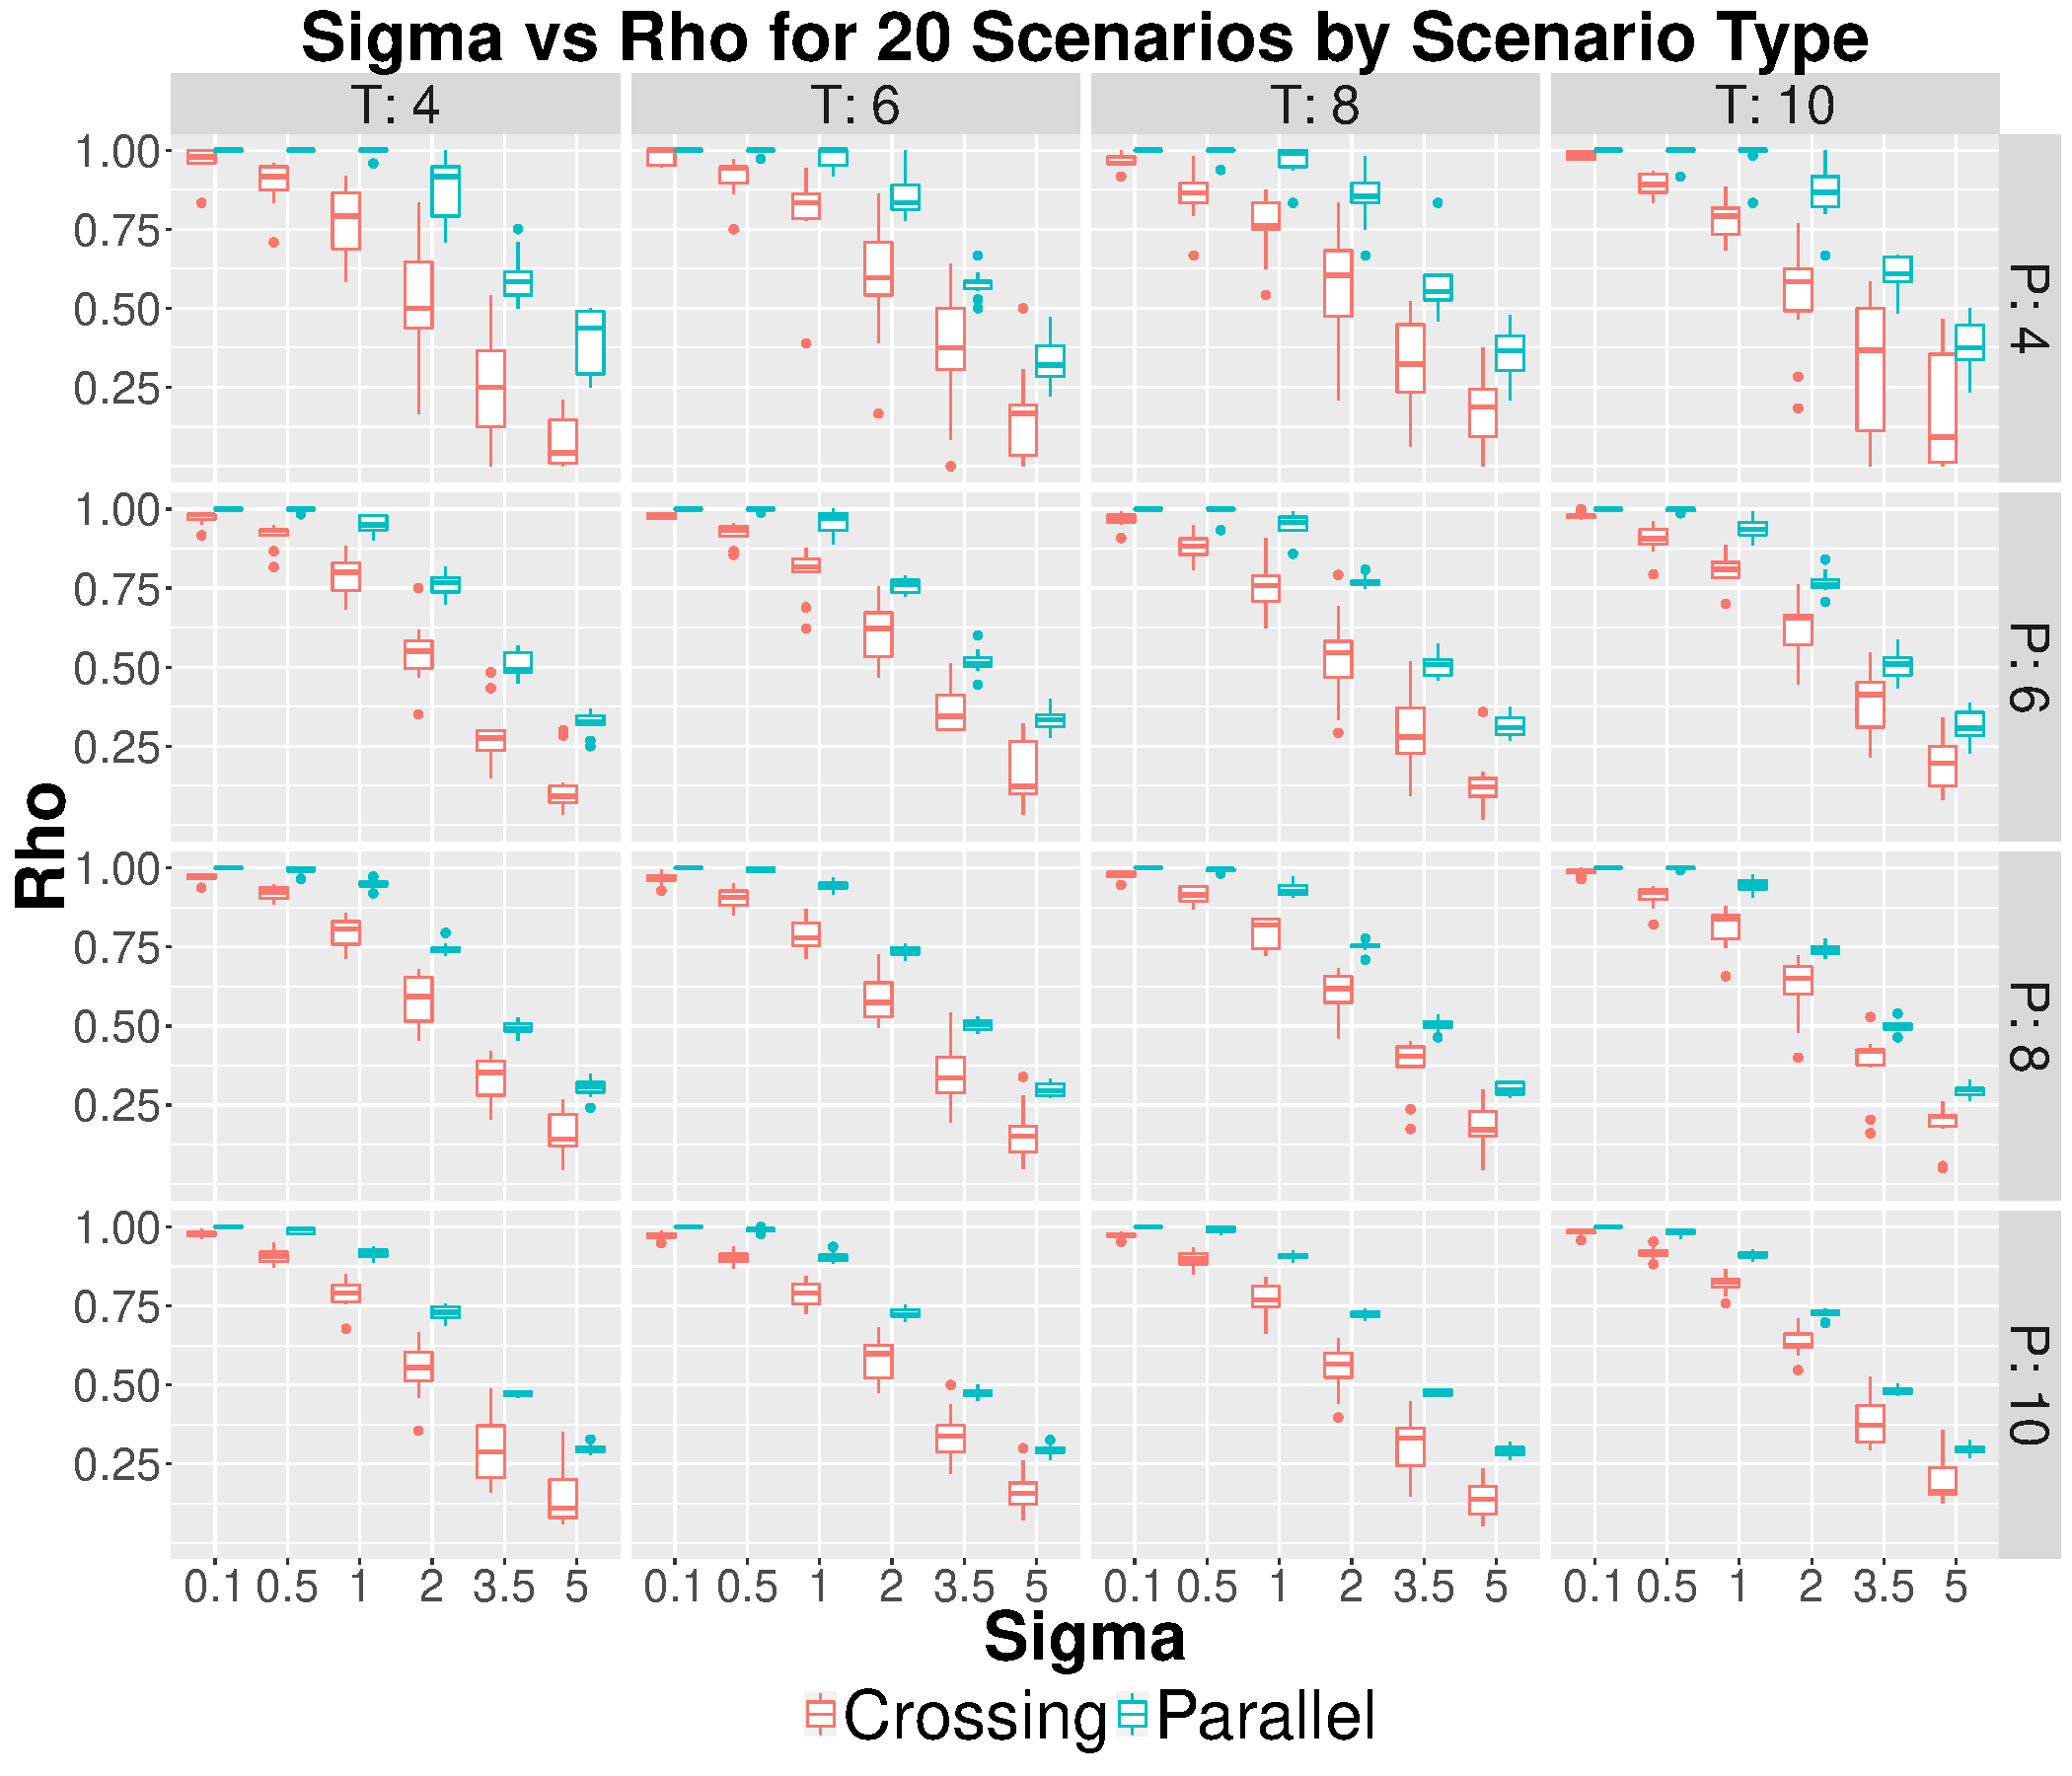
\includegraphics[width=\columnwidth]{../Figures//Sigma_vs_Rho}
    \caption{Relationship between $\sigma$ and $\rho$ summarized by scenario type for all 20 generated scenarios in this experiment.}
    \label{fig:Sigma_vs_Rho}
\end{figure}

Remember that higher values of $\rho$ indicate a higher proportion of detections within very close proximity to one another. We note that the parallel method of scenario generation clearly generates easier scenarios, as measured by $\rho$. This suggests that crossing scenarios, in general, may be more difficult to ascertain correct associations than parallel scenarios. In addition, we can conclude from Figure~\ref{fig:Sigma_vs_Rho} that $\sigma$ and $\rho$ are linearly correlated. Furthermore, we note that the the full range of $\rho$ from 0 to 1 is captured by a relatively smaller range of six values of $\sigma$. This result is beneficial to both scenario generation and complexity measuring because it suggests that $\sigma$ can be used in its natural domain of the data generation process, and $\rho$ can be back calculated as a measurement of difficulty for the data association problem. As a result, we gain a highly interpretable performance metric for the data association problem without sacrificing the ability to generate scenarios in their natural domain. 

\mysubsubsection{Basic Heuristic}
We transition to discuss performance of the heuristic, beginning with an examination of the experimental run times. Table~\ref{tab:Basic_heuristic_times} summarizes the minimum, mean, and maximum run times of the heuristic from the experiment for a single starting point, arranged by the number of targets ($P$) and number of scans ($T$). Times are shown in milliseconds. 

\begin{table}[ht]
\centering
\begin{tabular}{cc|ccc}
  \hline
   & & \multicolumn{3}{c}{Heuristic Run Times } \\
   & & \multicolumn{3}{c}{(in milliseconds)}\\
   P & T & Min & Mean & Max \\ 
  \hline
  \hline
   4 & 4 & 0.07 & 0.10 & 0.18 \\ 
   4 & 6 & 0.18 & 0.24 & 0.38 \\ 
   4 & 8 & 0.34 & 0.45 & 0.62 \\ 
   4 & 10 & 0.58 & 0.76 & 1.02 \\ 
   6 & 4 & 0.11 & 0.15 & 0.25 \\ 
   6 & 6 & 0.31 & 0.39 & 0.58 \\ 
   6 & 8 & 0.64 & 0.81 & 1.05 \\ 
   6 & 10 & 1.24 & 1.56 & 2.02 \\ 
   8 & 4 & 0.14 & 0.19 & 0.30 \\ 
   8 & 6 & 0.46 & 0.57 & 0.86 \\ 
   8 & 8 & 0.95 & 1.24 & 1.58 \\ 
   8 & 10 & 2.07 & 2.53 & 3.37 \\ 
   10 & 4 & 0.19 & 0.25 & 0.41 \\ 
   10 & 6 & 0.63 & 0.80 & 1.03 \\ 
   10 & 8 & 1.44 & 1.84 & 2.44 \\ 
   10 & 10 & 2.96 & 3.73 & 4.56 \\ 
   \hline
\end{tabular}
\caption{Heuristic run times (in milliseconds) for a single starting point.}
\label{tab:Basic_heuristic_times}
\end{table}

At a glance, it is evident that the heuristic scales more efficiently with increases in the number of targets than increases in the number of scans. Notice that the average run time roughly doubles with each addition of two scans, for a fixed number of targets. On the other hand, the average run time never increases more than 50$\%$ for an increase of two targets, given a fixed number of scans. Therefore, we conclude that the heuristic would be capable evaluating scenarios with a surprisingly large number of targets, but measures should be taken to avoid significant increases in the number of scans. 

Implementing the heuristic as sliding window algorithm would very likely mitigate this scaling effect in regards to $T$. Rather than solve all scans in a single batch at once, a sliding window algorithm solves a subset of scans, or a smaller window, and advances through all scans sequentially.  As the window progresses forward through the scans,``soft'' decisions are made meaning that the heuristic would begin with the decisions from the previous solution. As scans pass beyond the horizon and out of the sliding window, the decisions become fixed and we refer to them as ``hard" decisions. This process continues until all scans have been processed. The run times of a sliding window variant of the heuristic would not exhibit the curse of dimensionality in $T$ since the number of scans remains constant. Additionally, the heuristic is likely to produce higher quality solutions as a result of these ``soft" decisions of previous steps since it is starting from a solution which is likely to be better than a completely random solution. 

Furthermore, the full strength of the heuristic isn't realized until we remember that the heuristic is extremely parallelizable. By running the heuristic on several computers, we reduce the number of starting points needed for a single core. As a result, the heuristic can run several thousand starting points and still find solutions in fractions of seconds. To illustrate, say that we intend to run 50,000 heuristic starting points for a scenario with six targets and six scans. The average run time for a single starting point of this size is about 0.4 milliseconds. Running all of these starting points in sequence would require approximately 20 seconds of run time, however, the same amount of starting points parallelized onto 100 processors would only require a run time on the order of 0.2 seconds. Thus, the run time of the heuristic can be reduced to meet the efficiency needs of the system subject only to the limitation of available processors. 

We have seen that the heuristic scales efficiently in regards to the number of targets, and we have also seen the power of the heuristic when parallelized, but \textit{does the heuristic provide good feasible solutions to serve as a warm start to the MIO?} In order to answer this question appropriately, we compare the heuristic solution to the ideal solution, which as a reminder is the solution in which the data association problem is exactly correct. Toward this goal we compute the MIO objective value of both the heuristic solution and the ideal solution, and report the ratio of the first value to the second. Figure~\ref{fig:Basic_Heuristic_Objective} plots this ratio against $\sigma$.
\begin{figure}[ht]
  \centering
  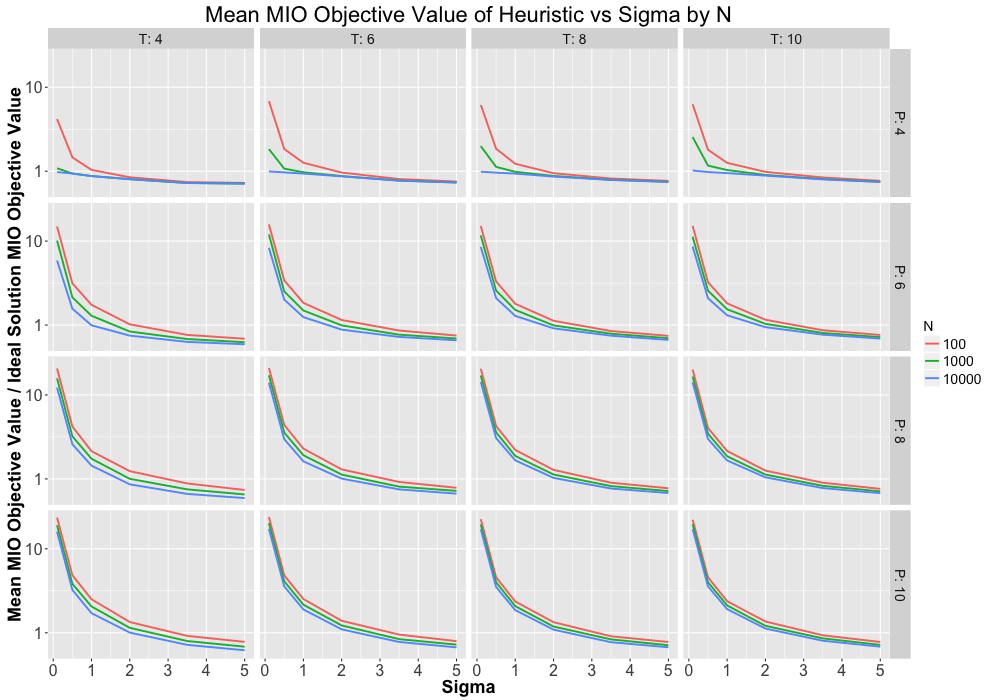
\includegraphics[width=\columnwidth]{../Figures/Basic_Heuristic_Objective}
  \caption{Quality of heuristic solution as compared to the ideal solution's MIO objective value summarized by number of starting points.}
  \label{fig:Basic_Heuristic_Objective}
\end{figure}

On the whole, we see that increasing the number of starting points improves the quality of heuristic solutions as compared to the ideal solution's MIO objective value, though the magnitude of improvement diminishes as the number of targets increases. Yet for scenarios with only four targets, we see that increasing the number of starting points has a significant effect. This suggests that in order to maintain solution quality, the number of necessary starting points increases with $P$, likely due to the exponential increase in combinatorial solutions as the number of targets increases. Additionally, there does not appear to be a significant loss in quality as the number of scans increases, suggesting that solution quality scales efficiently with increases in $T$. Altogether, this suggests that the heuristic solution quality scales better in regards to increases in $T$ than $P$. We remind the reader that this easily mitigated due to the fact that a very large number of starting points can be evaluated efficiently through the power of parallelization. 

Of important note, we also see that the heuristic outperforms the ideal solution's MIO objective value for larger values of $\sigma$. Remember that the ideal solution is simply ideal in the sphere of data association, while the MIO objective function serves to quantify solutions in regards to both data association and trajectory estimation simultaneously. This result suggests that the heuristic gives a better fit to the noise, but this fit does not necessarily lead to better estimated trajectories. With this in mind, we conclude that it may be necessary to tradeoff correct data associations in order to improve the trajectory estimation in cases of higher noise.

We continue our evaluation of the basic heuristic by measuring its performance on the data association problem. Figure~\ref{fig:Basic_Heuristic_Accuracy} plots the mean accuracy of each of the three quantities of starting points against $\rho$. 
\begin{figure}[ht]
  \centering
  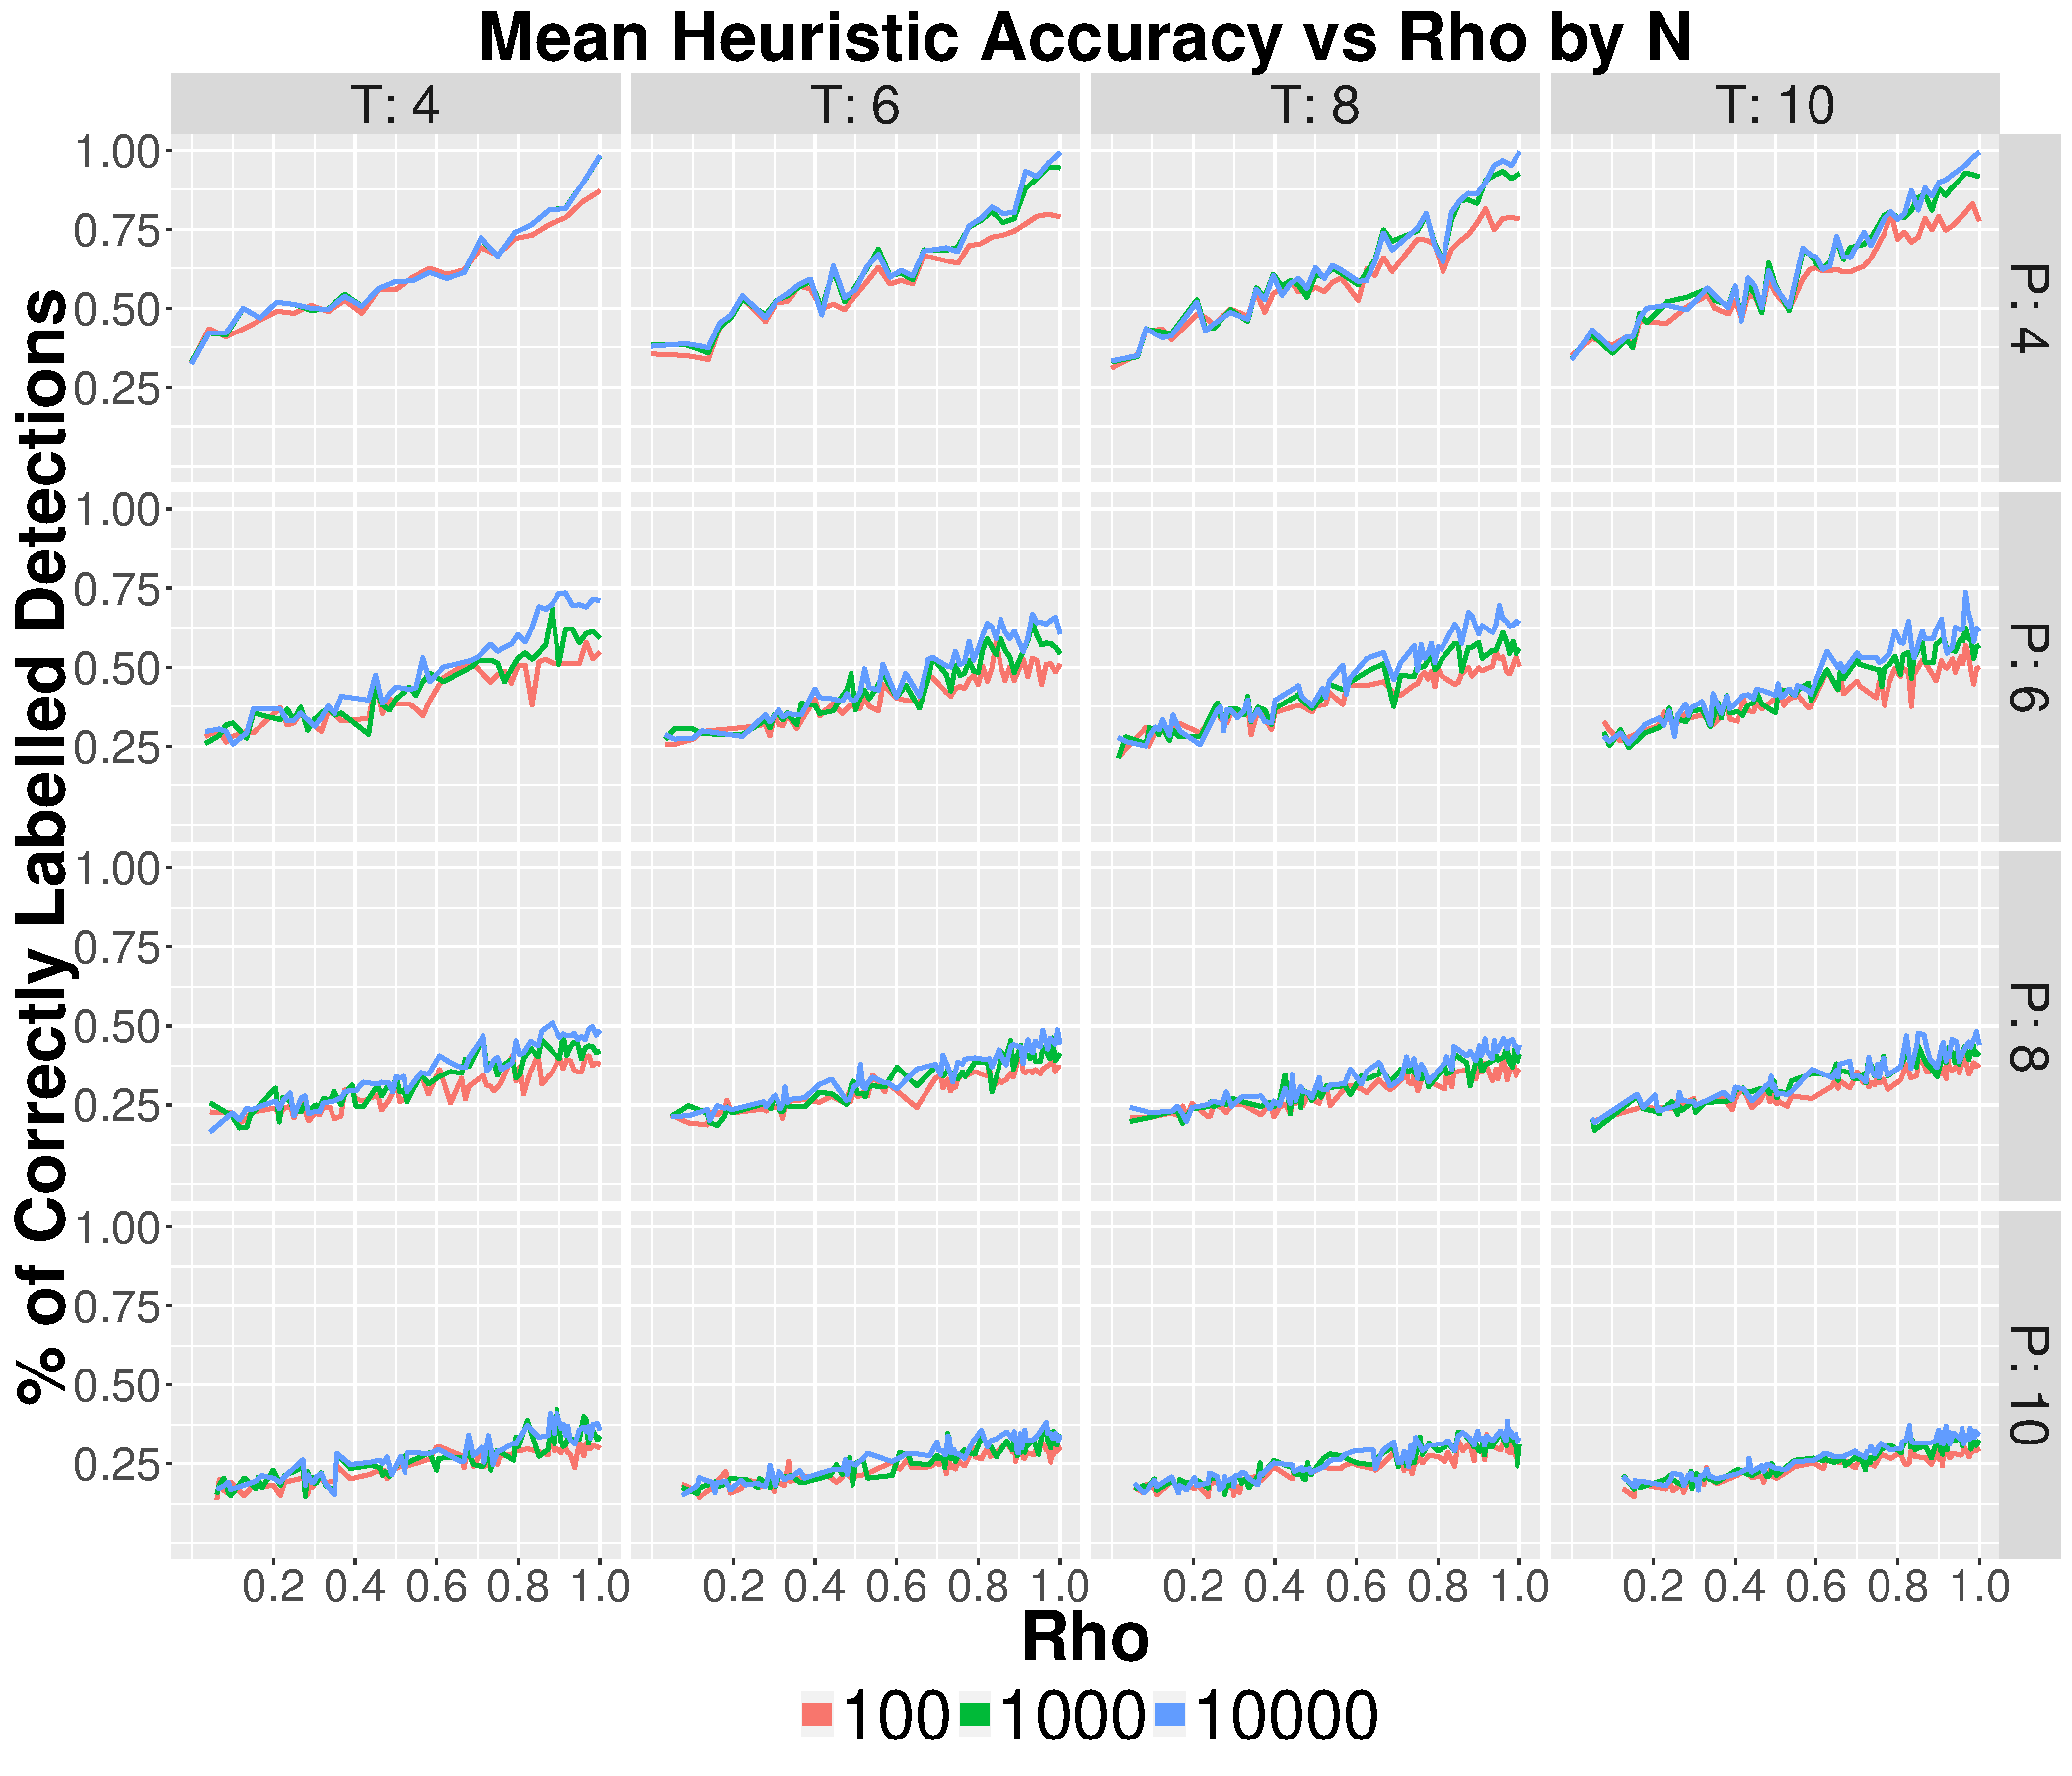
\includegraphics[width=\columnwidth]{../Figures/Basic_Heuristic_Accuracy}
  \caption{Accuracy of basic heuristic by number of heuristic starting points.}
  \label{fig:Basic_Heuristic_Accuracy}
\end{figure}

First of all, we see that the heuristic finds good solutions to the data association problem, especially for scenarios with fewer targets and higher values of $\rho$. While Figure~\ref{fig:Basic_Heuristic_Objective} may have instigated cause for concern of the scalability of the heuristic in regards to $P$, Figure~\ref{fig:Basic_Heuristic_Accuracy} reassures that the heuristic is adding value and finding nontrivial solutions, at least as it pertains to the data association problem. Perhaps this is further evidence that the ideal solution of perfect data associations does not always correspond to the best solution when balancing both data association and trajectory estimation.

Overall, we conclude that the heuristic run times scale especially well in regards to increases in the number of targets, though the solution quality may not scale quite as well. In any event, we have seen that there is not a significant difference in heuristic performance for the range of $N$ values that we explored. Therefore, for simplification as we move forward in our analysis, we will restrict our discussions of the heuristic to $N=1,000$. Next, we will see how the MIO performs. 

\mysubsubsection{Basic MIO}
We shift our focus to the MIO by first measuring its performance on the data association problem. Figure~\ref{fig:Basic_Accuracy_Summary} plots the mean accuracy of the MIO, initialized by the $N=1,000$ heuristic solutions, after 1,T, and 2T seconds against $\rho$. Note that we excluded the data for the MIO after 3T seconds for the sake of clarity as it showed little to no improvement over the MIO solution after 2T seconds. Also note that the ideal solution, which always achieves an accuracy of 1.0, has also been excluded. For comparison, we have included the accuracy of random solutions. 
\begin{figure}[ht]
  \centering  
  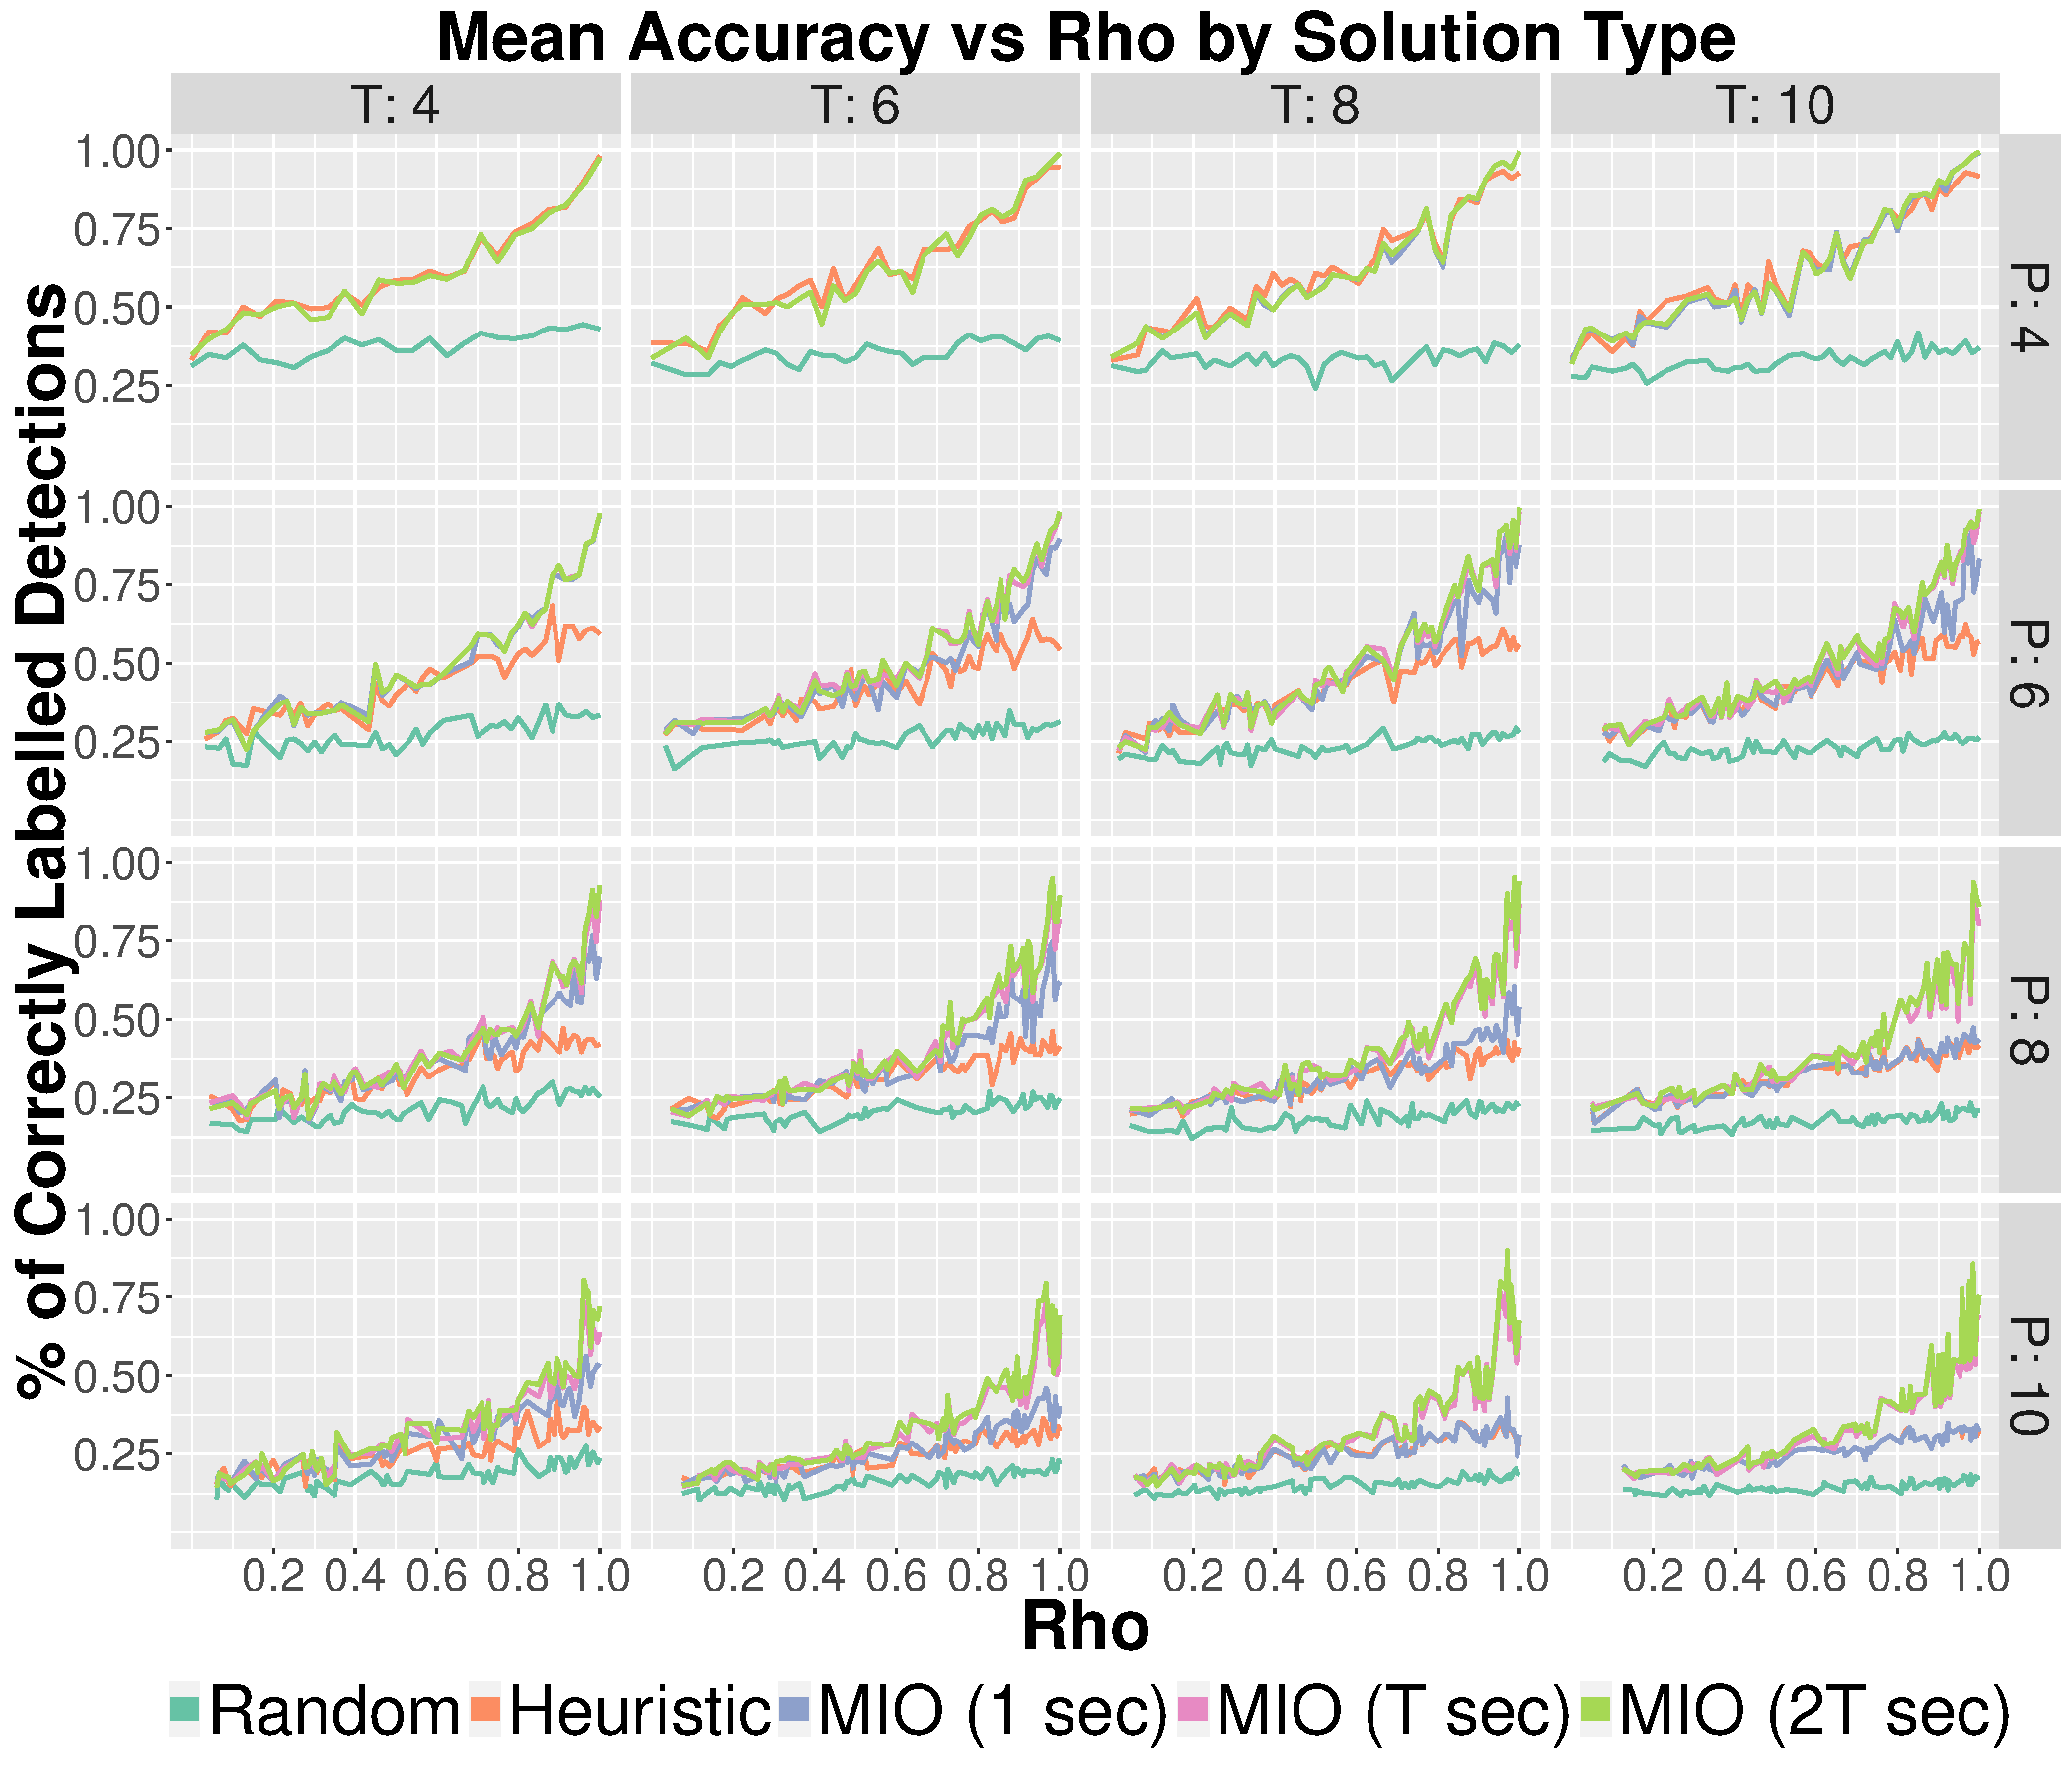
\includegraphics[width=\columnwidth]{../Figures/Basic_Accuracy_Summary}
  \caption{Accuracy of MIO compared against the heuristic and a randomized solution.}
  \label{fig:Basic_Accuracy_Summary}
\end{figure}

The MIO finds high quality solutions to the data association problem, and it appears to scale fairly well in regards to increases in both $P$ and $T$. For all scenarios with eight or fewer targets, accuracy tops out at or near 1.0, and reduces to about 0.85 for ten target scenarios. Furthermore, scenarios with ten scans appear to slightly outperform scenarios with only four scans, suggesting that additional scans benefit the MIO solution quality, likely due to the added information gathered from an increase in the number of detections. 

While not seen in Figure~\ref{fig:Basic_Accuracy_Summary}, we note that for scenarios with four targets, many of the MIO solutions were actually proven to be the optimal solution. The fact that the heuristic performance is almost identical to the MIO again suggests that the heuristic finds high quality solutions. This is further supported by the fact the heuristic performs almost as well as the MIO after 1 second even in scenarios with ten targets. Equally as important, Figure~\ref{fig:Basic_Accuracy_Summary} shows that in nearly all scenarios, the MIO achieves its best or near best solutions after $T$ or fewer seconds, suggesting the usefulness of the MIO as an online algorithm with a sliding window. As mentioned previously in regards to the heuristic, a sliding window algorithm would make decisions on a subset of scans, and these decisions will be fixed before accepting a new set of scans. In regards to the MIO, this would be implemented by adding constraints to restrict the values of $y_{itj}$ to match that of the subsetted solution. The fact that the MIO finds very good solutions in $T$ or fewer seconds means that a sliding window algorithm would be able to solve each subset in real time before advancing to the next subset of scans. Furthermore, the MIO would likely benefit from the fixed decisions of the preceding windows, since this is added knowledge that has not utilized by our approaches.

Next, we evaluate the performance of the basic heuristic and MIO through the lens of trajectory estimation. As discussed previously, we are interested in comparing $\delta$, our proxy for ground track error, against $\sigma$, our measure of difficulty for trajectory estimation, in order to analyze performance of in the sphere of estimation. Figure~\ref{Fig:Basic_Delta_Summary} plots $\sigma$ against $\delta$ for each of the solution types. In addition to the random solution shown on the previous plot, we also add a comparison to the ideal solution, as previously defined.
\begin{figure}[ht]
  \centering
  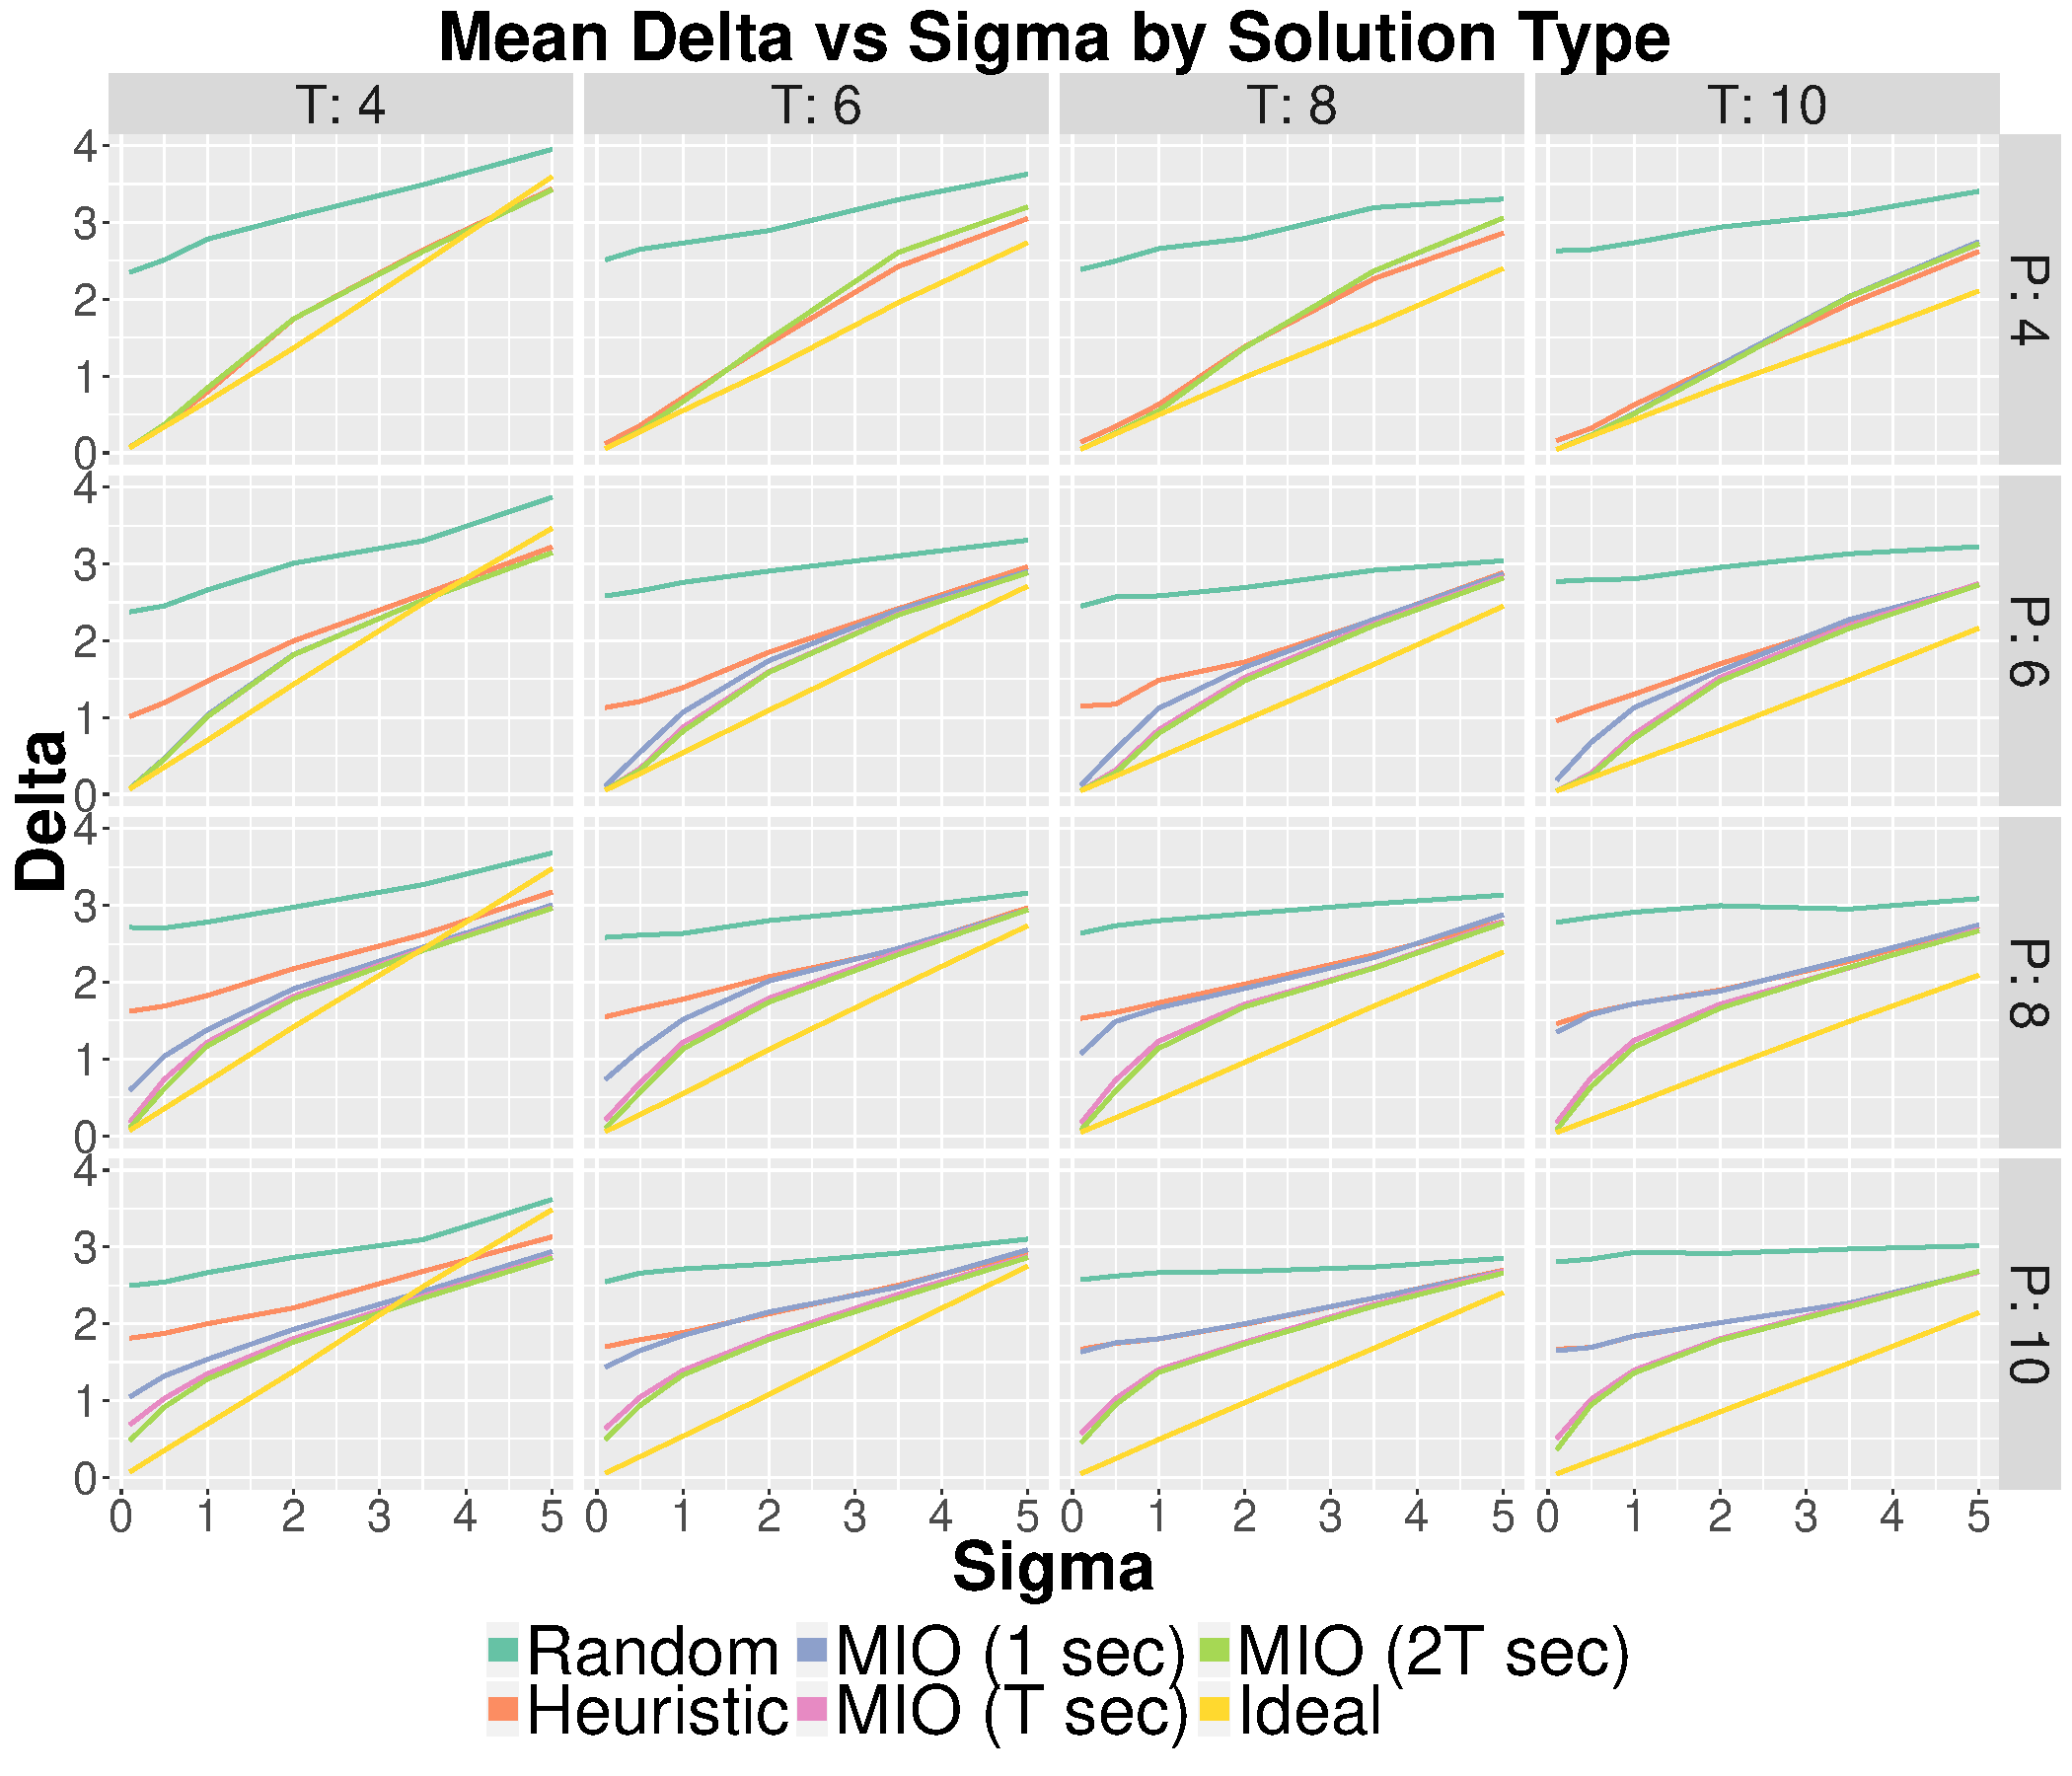
\includegraphics[width=\columnwidth]{../Figures/Basic_Delta_Summary}
  \caption{Trajectory estimation performance}
  \label{Fig:Basic_Delta_Summary}
\end{figure}

Remember that lower values of delta correspond to trajectory estimations that are closer to that of the true ground track. We see that the performance of the heuristic converges to that of the MIO for scenarios with few targets, as well as for large values of $\sigma$. Additionally, we see that as the number of targets increases we begin to see stronger improvements by the MIO over the heuristic. Interestingly, we see that for the scenarios with the largest number of targets and scans, the MIO after one second is not much better than the heuristic. While the MIO after T seconds provides significant improvement over that of the heuristic and MIO after 1 second, there is little further improvement in running the MIO for 2T seconds. 

Again, we see that occasionally the heuristic and/or MIO outperform(s) the ideal solution, especially for scenarios with only four scans. This effect increases as the value of $\sigma$ increases. This result suggests that as the number of scans approaches infinity, the estimated trajectories of the ideal solution approaches the true ground track. Put differently, as more and more data is known, it becomes easier to estimate the trajectories even in the event of large noise, and so the trajectory estimates that result from the ideal solution converges to the true ground track. 

In summary, we have shown that in the case of no detection ambiguity, the heuristic is scalable, particularly in regards to increases in the number of targets, and it finds high quality solutions in milliseconds. The MIO is also scalable, appearing relatively robust to both increases in the amount of targets and scans. Both approaches show promising signs for use in a sliding window algorithm.

\mysubsection{Scenarios with Detection Ambiguity}
Here we extend our discussion to analyze the performance of our methods on scenarios with detection ambiguity. We first summarize our experimental methods before discussing performance of both the robust heuristic and the robust MIO in the spheres of both the data association and trajectory estimation problems.

This experiment serves as an extension of the basic one, in order to test the performance of our algorithms under detection ambiguity. We use the same scenarios generated from the basic experiment, however due to the additional difficulty inherent with detection ambiguity, we limit the range of signal noise to $\sigma \in \{0.1,0.5,1.0,2.0\}$, choosing to exclude the extreme cases of signal noise. In addition, we simulate both missed detections and false alarms. A detection is removed with probability, $\gamma$, and we consider $\gamma \in \{0.2,0.15,0.1,0.05\}$. We do not allow empty scans. For each scan, we generate false alarms according to a poisson distribution with parameter, $\lambda$, and false alarm locations are randomly selected uniformly within the state space. We consider $\lambda \in \{0.1,0.5,0.1,2.0\}$. The false alarms are then added to $\mathcal{X}_{t}$ and the detection order of $\mathcal{X}_{t}$ is randomly shuffled in the same manner as the first experiment. 

Once the data has been generated, we follow the same sequence of steps as outlined for the basic experiment, running the heuristic first and then feeding the solution into the MIO as a warm start. Note that the heuristic is only initialized with 1,000 starting points, as determined from the results of the basic experiment. Once again, the optimization process was set to terminate after 3T seconds, with solutions collected at intervals of $\{1,T,2T,3T\}$ seconds. Prior to the running of this experiment, we performed a mini experiment and used the results to tune the penalties $\theta$ and $\phi$. A summary of the exact penalties used along with an explanation of the insight behind them, can be found in Appendix~\ref{app:Penalty_Appendix}. 

\mysubsubsection{Robust Heuristic} Table~\ref{tab:Robust_heuristic_times} summarizes the minimum, mean, and maximum run times of the heuristic from the robust heuristic for a single starting point, arranged by the number of estimated targets ($P_{\text{est}}$) and number of scans ($T$). Times are shown in milliseconds. 

\begin{table}[ht]
\centering
\begin{tabular}{cc|ccc}
  \hline
   & & \multicolumn{3}{c}{Heuristic Run Times } \\
   & & \multicolumn{3}{c}{(in milliseconds)}\\
   $ P_{\text{estimated}}$ & T & Min & Mean & Max \\ 
  \hline
  \hline
  2 & 4 & 0.15 & 0.23 & 0.41 \\ 
  2 & 6 & 0.42 & 0.56 & 0.93 \\ 
  2 & 8 & 0.77 & 1.04 & 2.24 \\ 
  2 & 10 & 1.27 & 1.73 & 20.23 \\ 
  4 & 4 & 0.15 & 0.34 & 1.04 \\ 
  4 & 6 & 0.50 & 0.94 & 2.69 \\ 
  4 & 8 & 1.09 & 1.88 & 3.87 \\ 
  4 & 10 & 2.12 & 3.25 & 13.51 \\ 
  6 & 4 & 0.14 & 0.42 & 0.96 \\ 
  6 & 6 & 0.57 & 1.29 & 4.45 \\ 
  6 & 8 & 1.33 & 2.66 & 75.28 \\ 
  6 & 10 & 2.53 & 4.61 & 18.69 \\ 
  8 & 4 & 0.16 & 0.50 & 1.10 \\ 
  8 & 6 & 0.60 & 1.59 & 3.46 \\ 
  8 & 8 & 1.38 & 3.37 & 6.87 \\ 
  8 & 10 & 2.63 & 5.84 & 12.40 \\ 
  10 & 4 & 0.18 & 0.55 & 1.10 \\ 
  10 & 6 & 0.72 & 1.82 & 3.98 \\ 
  10 & 8 & 1.53 & 3.96 & 8.18 \\ 
  10 & 10 & 3.42 & 6.93 & 13.93 \\ 
  12 & 4 & 0.16 & 0.56 & 0.99 \\ 
  12 & 6 & 0.99 & 1.95 & 3.96 \\ 
  12 & 8 & 1.74 & 4.33 & 8.69 \\ 
  12 & 10 & 3.40 & 7.71 & 15.10 \\ 
   \hline
\end{tabular}
\caption{Robust heuristic run times (in milliseconds) for a single starting point.}
\label{tab:Robust_heuristic_times}
\end{table}

\textit{How do the run times of the robust heuristic compare to those of the basic heuristic?} The robust heuristic evidently requires longer run times. Comparing Table~\ref{tab:Basic_heuristic_times} and Table~\ref{tab:Robust_heuristic_times} we see that robust run times for four estimated targets are roughly four times as long as corresponding run times in the basic heuristic for a fixed number of scans. However, the magnitude of this effect appears to decay as the number of targets increases. Comparing equivalent scans for eight targets in both heuristics, we see that the robust heuristic times are about twice that of the basic heuristic. This increase in run times was expected due to the increase in combinatorial solutions in the robust heuristic over the basic heuristic. Yet the robust heuristic is still highly parallelizable, which means that much of these effects can be mitigated through the 

\textit{How does the robust heuristic scale in regards to $P_{\text{est}}$ and $T$?} The robust heuristic scales extremely well with respect to $P_{\text{est}}$ More importantly, scalability actually improves as the number of estimated targets and scans increases. To demonstrate, increasing from two to six estimated targets for four scans roughly doubles the run time, while increasing from eight to twelve estimated targets for four scans increases the run time by only 12\%. This result suggests that the robust heuristic run times scale efficiently in regards to $P_{\text{est}}$. However, the robust heuristic does not scale as well in regards to $T$, roughly doubling in run time with each increase of two scans for a fixed $P_{\text{est}}$. 

\textit{How does the robust heuristic scale in comparison to the basic heuristic?} By comparison, the robust heuristic scales about the same as the basic heuristic in regards to the number of targets, but may scale equally or slightly worse than the basic heuristic in regards to the number of scans. However, this effect can be mitigated through the advantage of parallelization, which we continue to stress is critical to the success of the heuristic. 

\mysubsubsection{Estimating the Number of Targets}
Perhaps the most important goal of a MTT algorithm in the case of detection ambiguity is to correctly estimate the number of targets. Hence, we begin our analysis be evaluating the difference between the true and estimated number of targets. Explicitly, we define:
\begin{align}
	P_{\text{diff}} = P_{\text{true}} - P_{\text{est}},
\end{align}
where $P_{\text{est}}$ is the number of estimated targets and $ P_{\text{true}}$ is the number of true targets. Note that $P_{\text{difference}} = 0$ indicates that the algorithms have correctly estimated the number of targets. When $P_{\text{difference}} < 0$, we the algorithm has overestimated the number of targets, whereas when $P_{\text{difference}} > 0$, the algorithm has underestimated the number of targets. Figure~\ref{fig:Robust_4_8_Histogram} plots the distribution of $P_{\text{diff}}$ for scenarios with four targets and eight scans, and for comparison, Figure~\ref{fig:Robust_8_8_Histogram} plots the same result for scenarios of eight targets and eight time scans. 
\begin{figure}[ht]
  \centering
  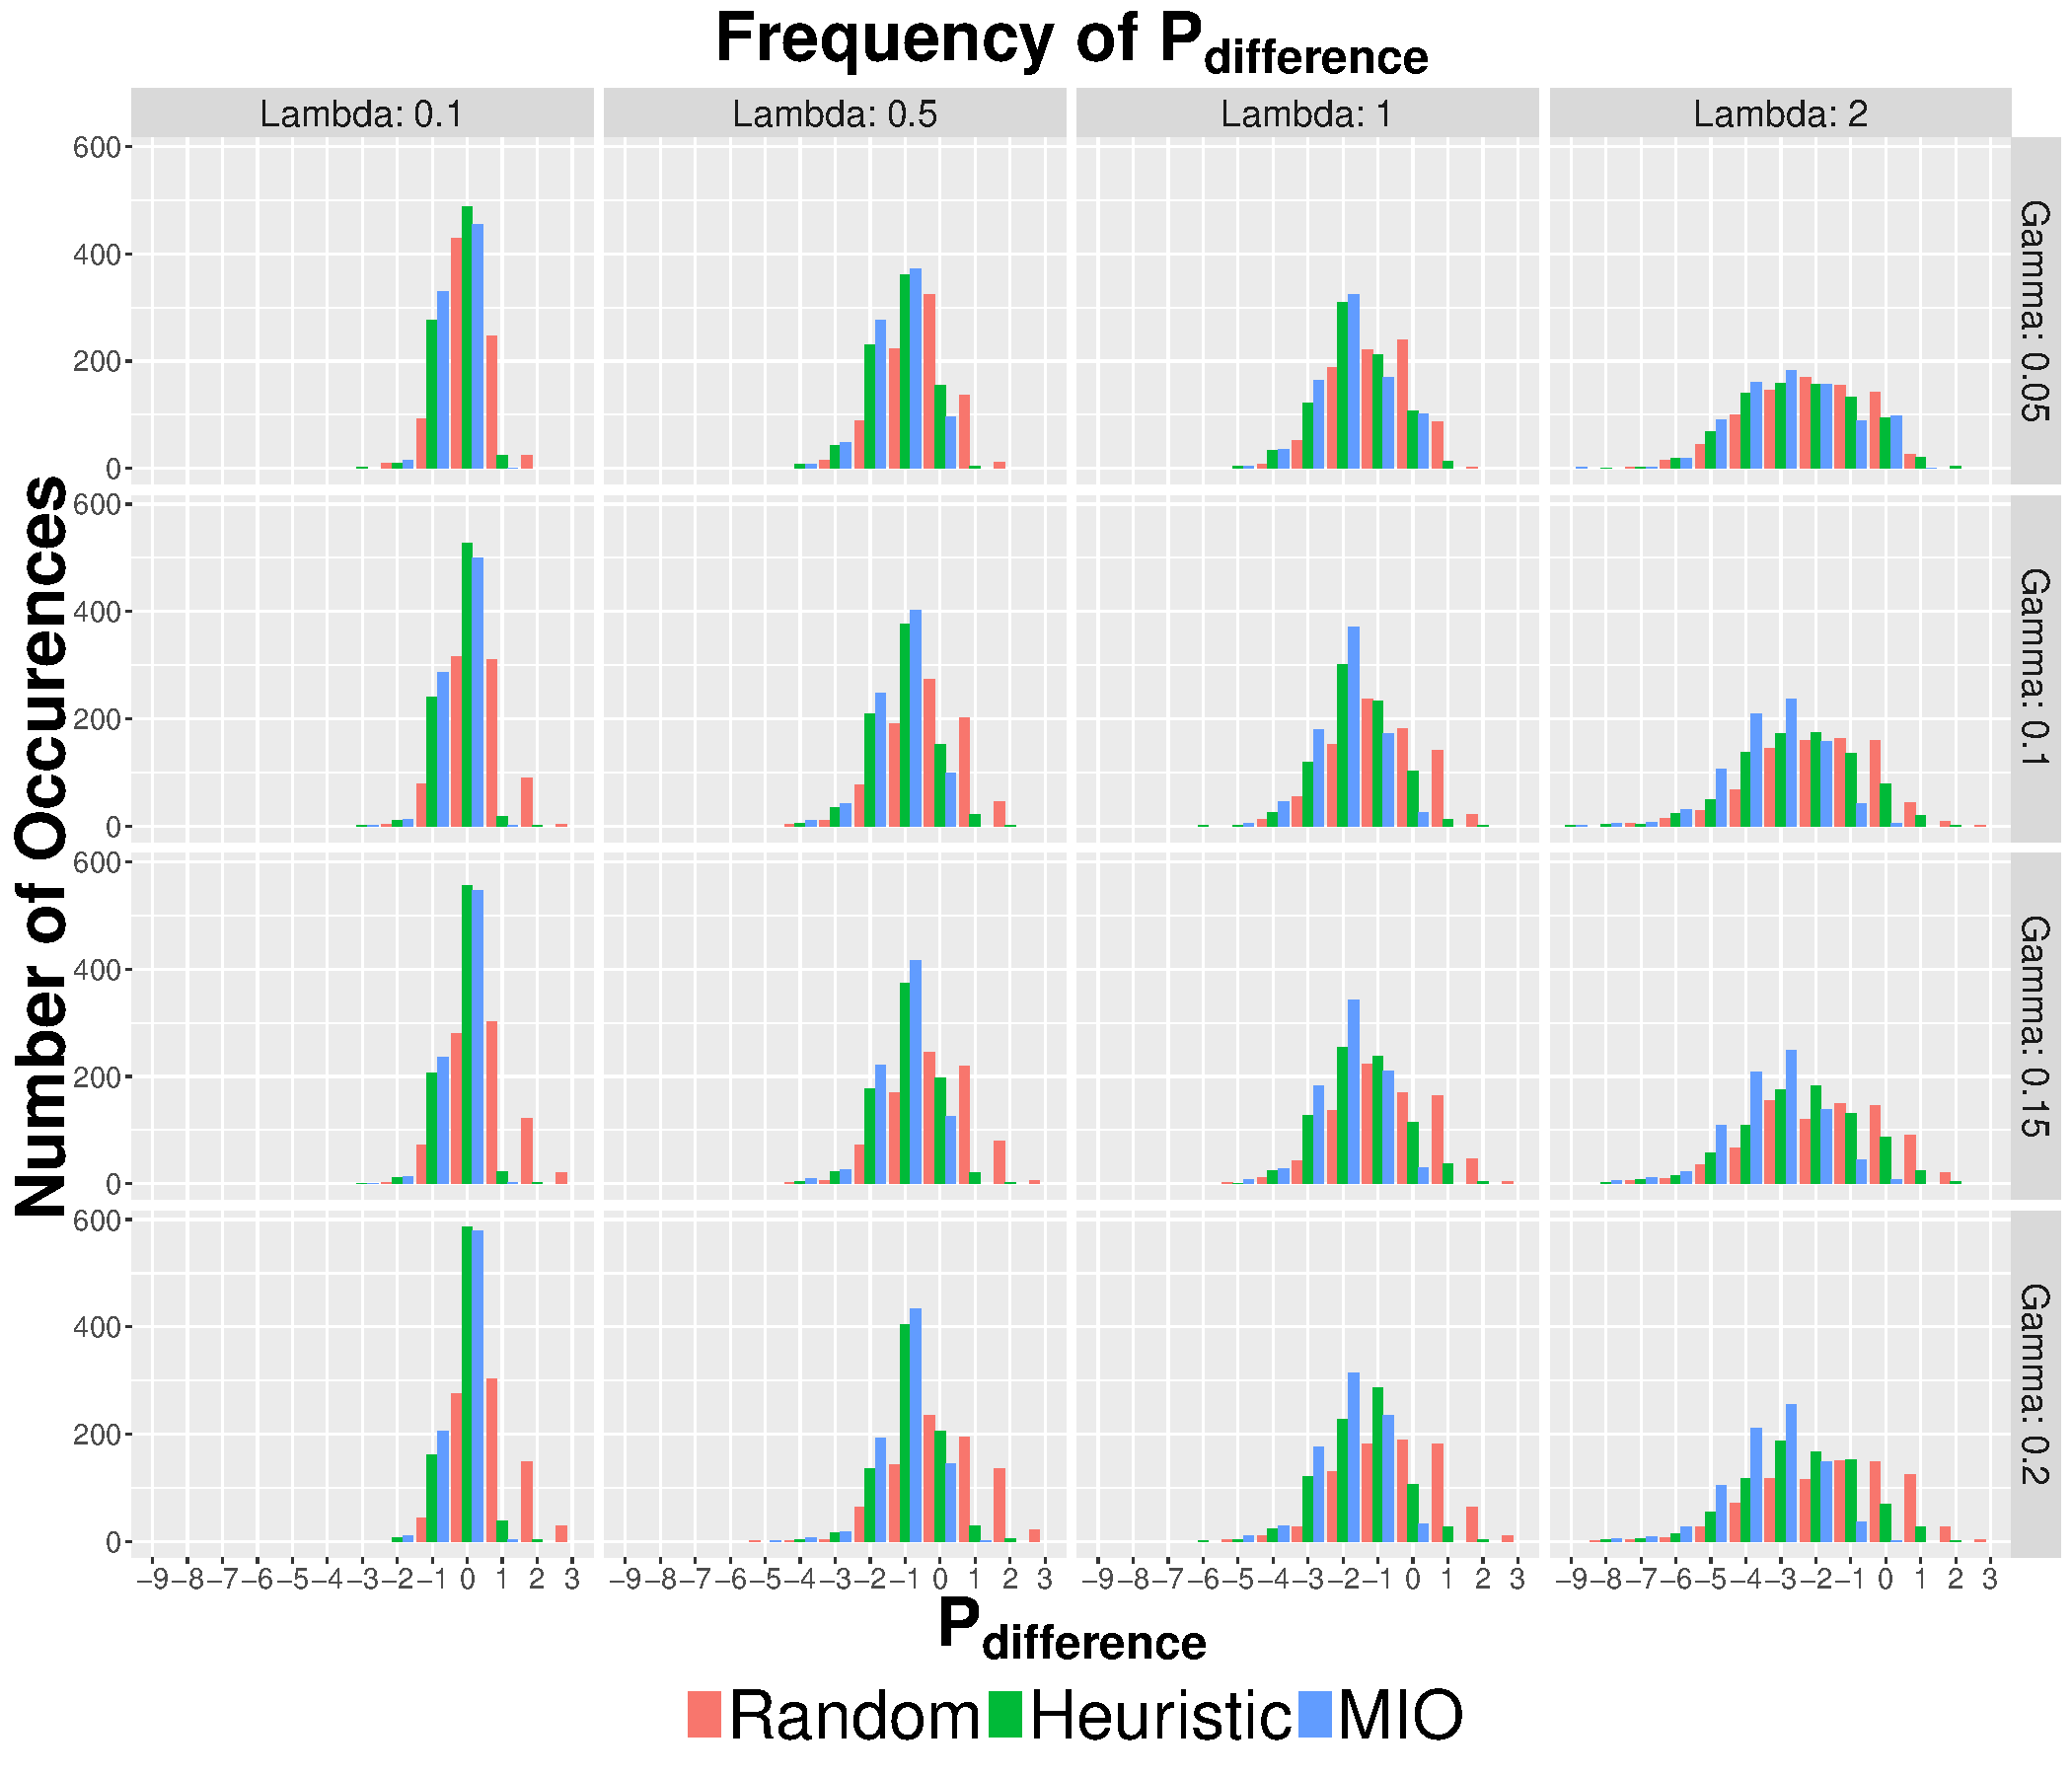
\includegraphics[width=\columnwidth]{../Figures/4_8_Histogram}
  \caption{Distribution of the difference in true and estimated number of targets for scenarios with 4 targets and 8 scans, arranged by $\gamma$ and $\lambda$.}
  \label{fig:Robust_4_8_Histogram}
\end{figure}
\begin{figure}[ht]
  \centering
  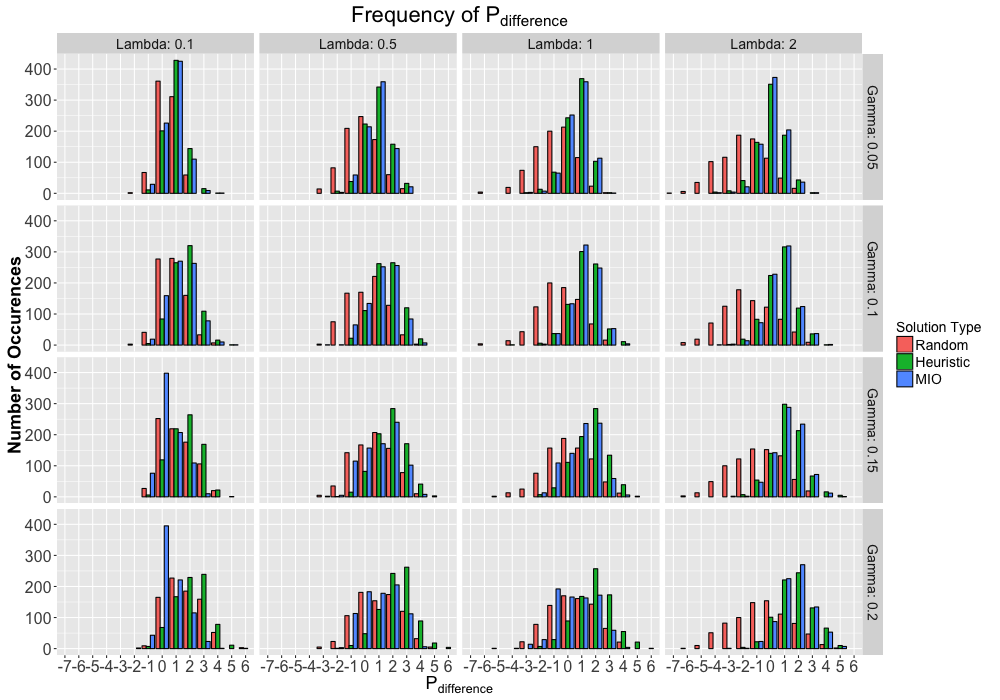
\includegraphics[width=\columnwidth]{../Figures/8_8_Histogram}
  \caption{Distribution of the difference in true and estimated number of targets for scenarios with 8 targets and 8 scans, arranged by $\gamma$ and $\lambda$.}
  \label{fig:Robust_8_8_Histogram}
\end{figure}

We see that both the robust heuristic and the robust MIO estimate the number of targets correctly a high proportion of the time in the scenario with four targets, particularly for smaller values of $\lambda$. As $\lambda$ increases, though, both algorithms tend to underestimate. The same trend persists in the larger scenario. This suggests that either 1) the false alarm penalty needs further tuning and likely was not set high enough in the experiment or 2) the missed detection penalty set too high. In the case where $\theta$ is set too low, the algorithms would prefer to classify detections as false alarms rather than create additional trajectories for the detections. In the case of $\phi$ set too high, the algorithms would opt out of creating additional trajectories in order to decrease the need to fill smaller scans with missed detections. Furthermore, because the effect of underestimation is more prominent in the scenario with more targets, we conclude that both penalties should probably take into account the number of targets that it is currently estimating.

\mysubsubsection{Data Association}
Knowing that we tend to underestimate the number of targets with the given penalties, we move on in our analysis to measuring the accuracy of our robust approaches. Figures~\ref{fig:Robust_4_8_Accuracy} and~\ref{fig:Robust_8_8_Accuracy} plot the accuracy performance metric against the difficulty metric, $\rho$, for scenarios of four and eight targets, respectively. Both scenarios have eight scans and both Figures have been arranged by $\gamma$ and $\lambda$.
\begin{figure}[ht]
  \centering
  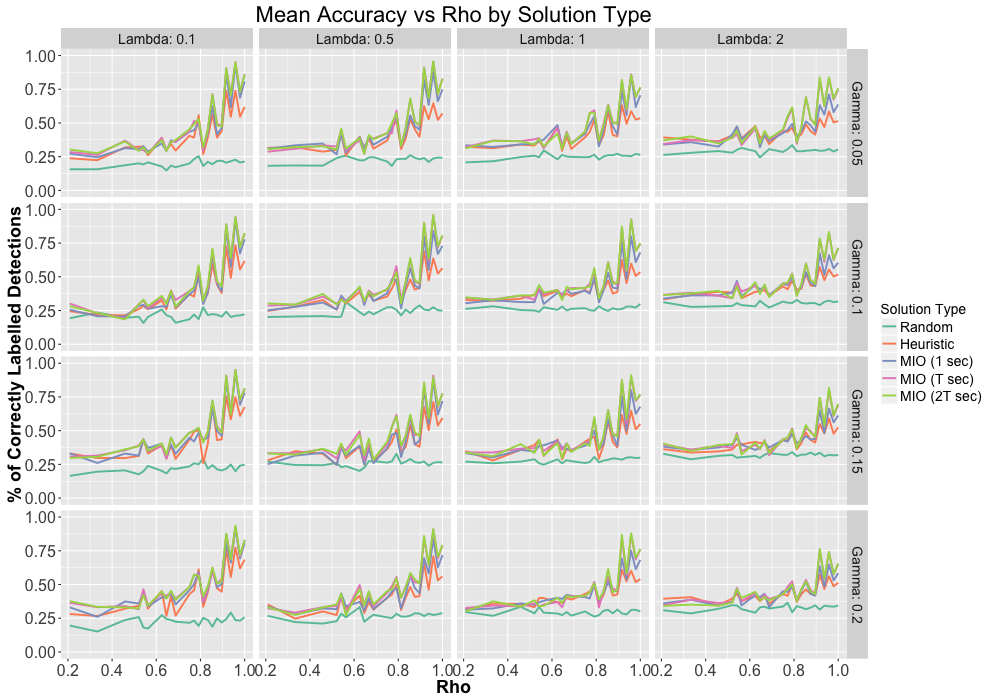
\includegraphics[width=\columnwidth]{../Figures/4_8_Accuracy}
  \caption{Accuracy of robust heuristic and MIO as compared to random solutions for scenarios of 4 targets and 8 scans, arranged by $\gamma$ and $\lambda$.}
  \label{fig:Robust_4_8_Accuracy}
\end{figure}

\begin{figure}[ht]
  \centering
  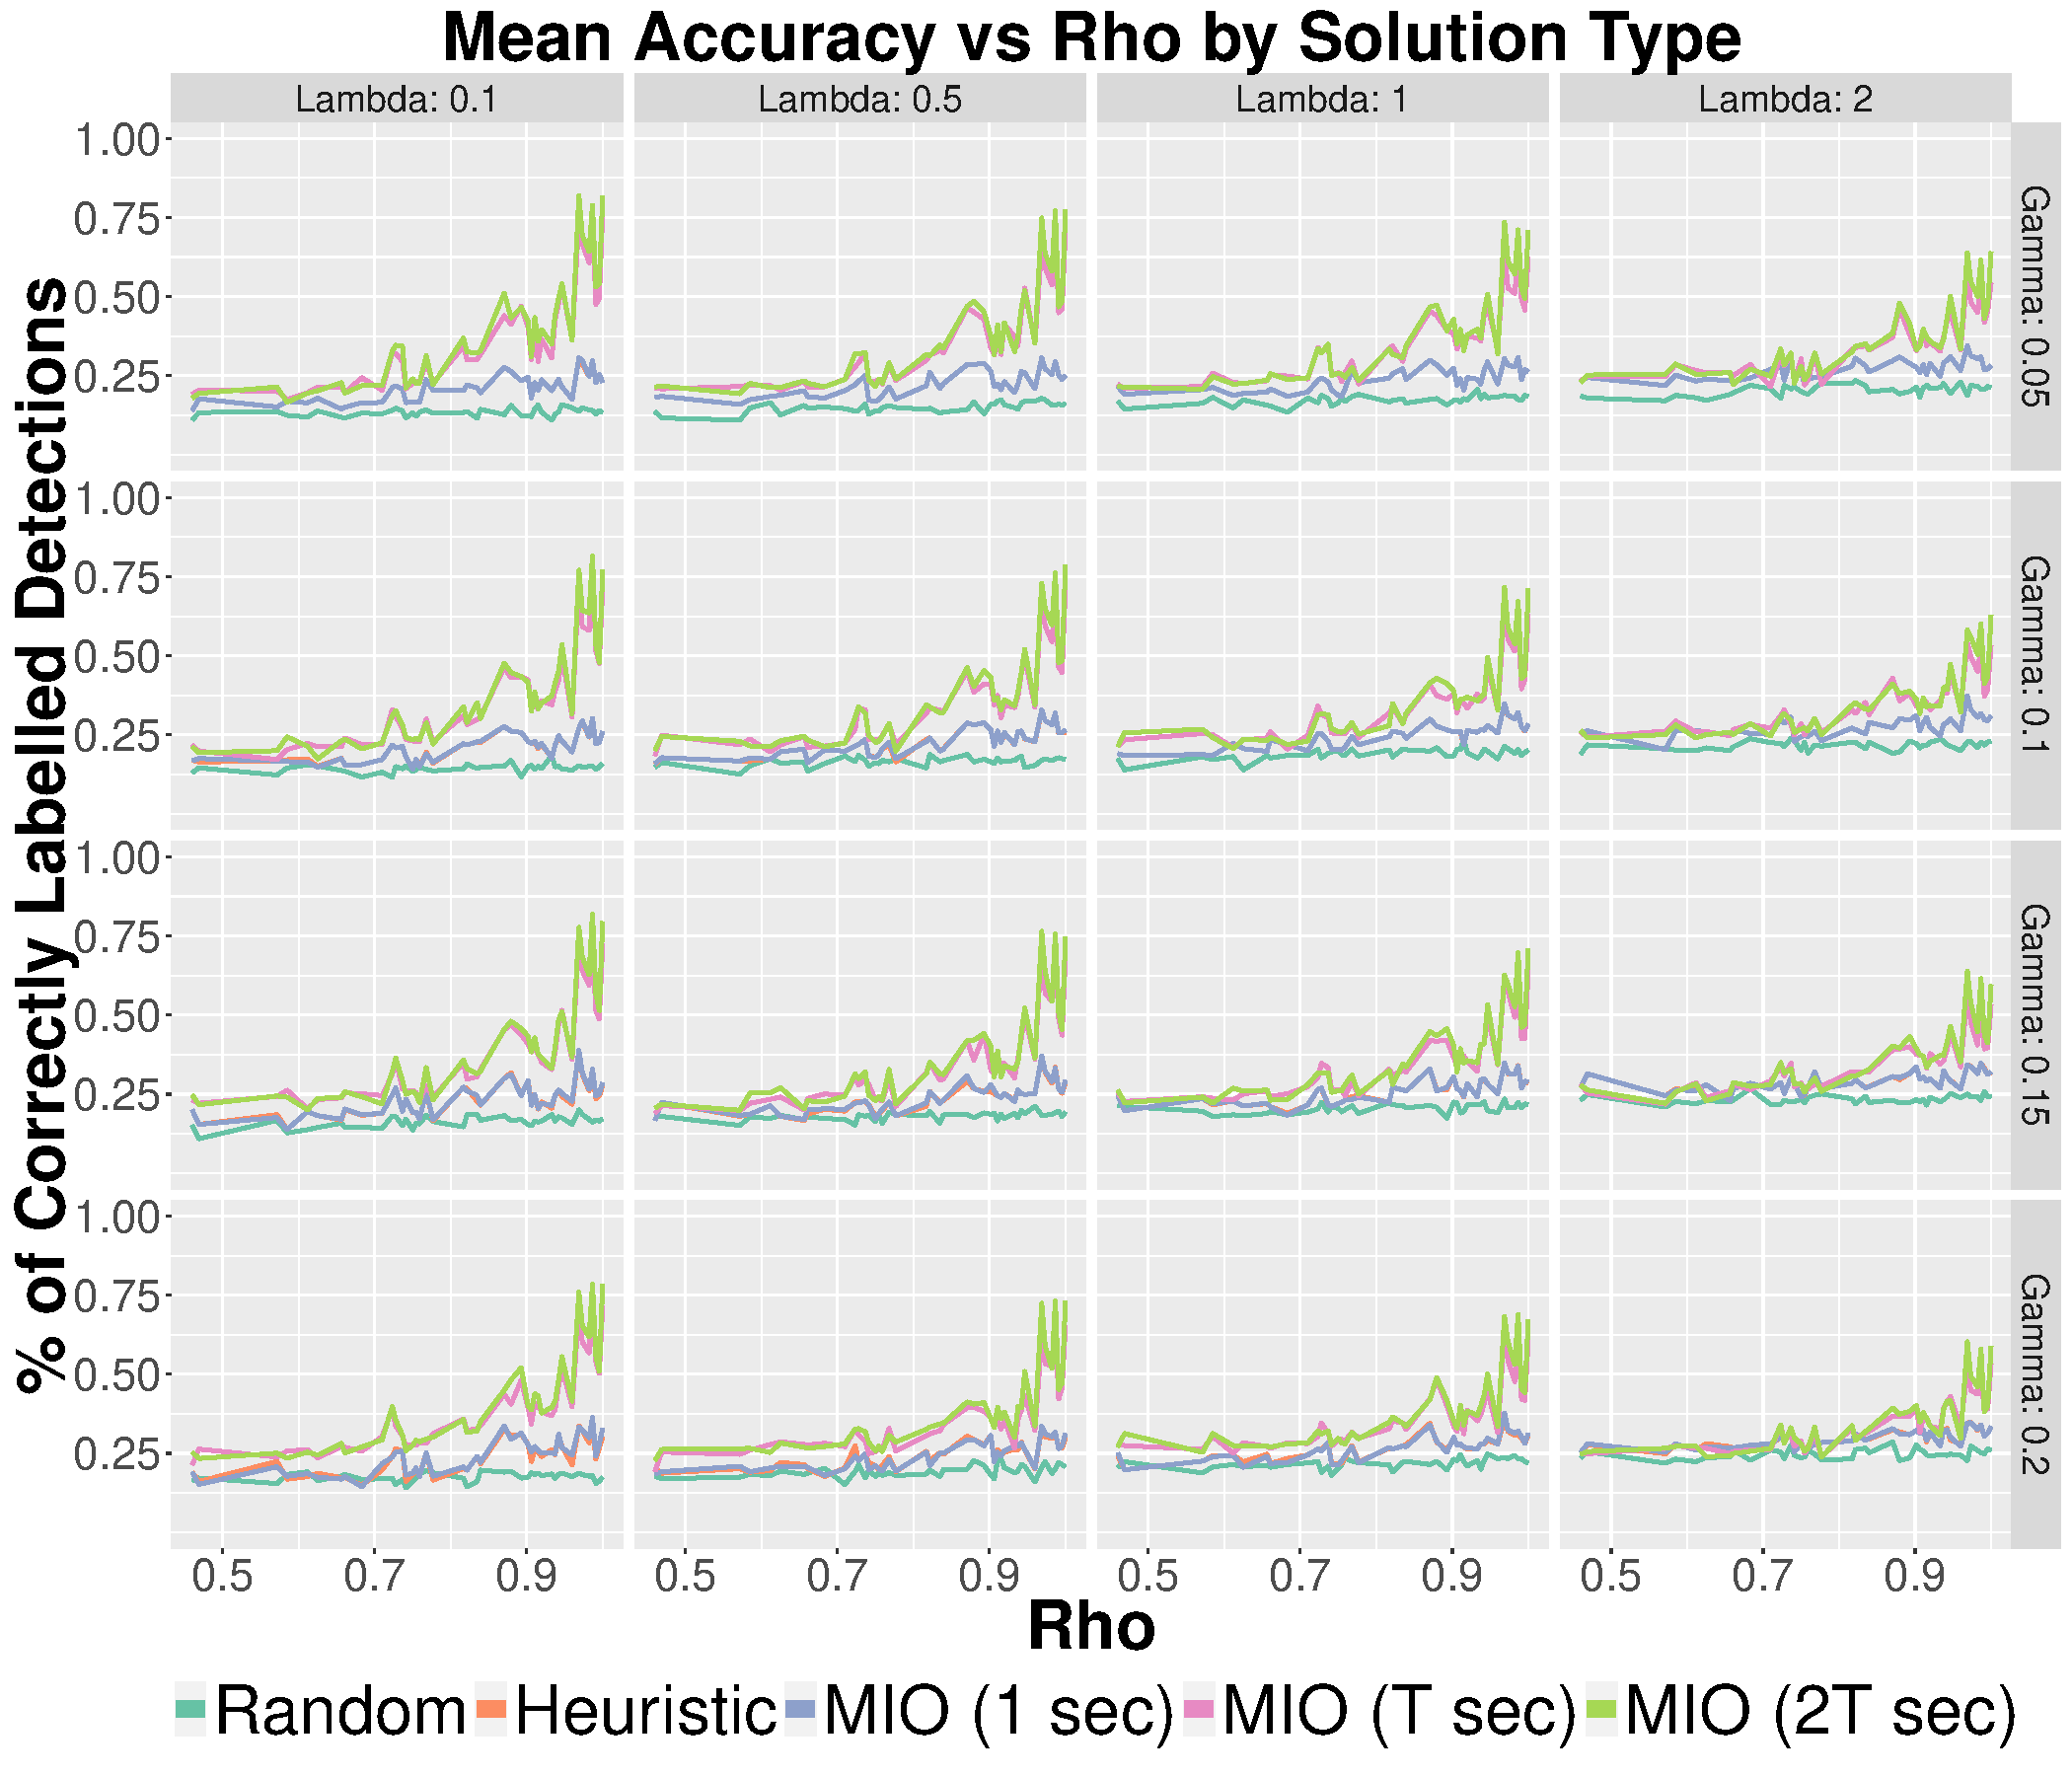
\includegraphics[width=\columnwidth]{../Figures/8_8_Accuracy}
  \caption{Accuracy of robust heuristic and MIO as compared to random solutions for scenarios of 8 targets and 8 scans, arranged by $\gamma$ and $\lambda$.}
  \label{fig:Robust_8_8_Accuracy}
\end{figure}

Similar to the performance of the basic heuristic, we again see that the robust heuristic improves greatly over that of a random solution, and the MIO offers even further improvement. Again, we seeing that running the MIO for 1 second offers significant improvements over the heuristic, and running the MIO for T seconds offers further improvement. However, running the MIO for 2T seconds offers little to no further improvement. Again, these results support the use of the MIO in an online algorithm with a sliding window as mentioned previously. 

Comparing Figure~\ref{fig:Robust_4_8_Accuracy} with the 4 target and 8 scan element of Figure~\ref{fig:Basic_Accuracy_Summary}, we see only a slight decrease in performance when $\gamma = 0.05$ and $\lambda=0.1$. This is an important result because we no longer know the number of targets in the robust case, yet we achieve almost the same levels of accuracy. Furthermore, both Figure~\ref{fig:Robust_4_8_Accuracy} and Figure~\ref{fig:Robust_8_8_Accuracy} show that the robust algorithms are more robust to decreases in the detection probability $\gamma$ than to increases in the false alarm rate $\lambda$. We conclude that the robust approaches are more sensitive to changes in the false alarm rate, in particular when it comes to making data associations. 

We have shown that both the heuristic and the MIO tend to underestimate the number of targets, due to the chosen penalties. We have also shown that accuracy degrades as the false alarm rate increases. This is likely not a coincidence. It is probable that as a result of underestimation, in which fewer trajectories are generated, there is a higher rate of misclassification of detections as false alarms, which in turn directly leads to a reduced accuracy. Therefore, it is a promising result to see accuracies above 75\% in Figure~\ref{fig:Robust_8_8_Accuracy}, even when Figure~\ref{fig:Robust_8_8_Histogram} suggests overestimation. It is entirely possible that further parameter tuning or introducing more complex penalties would lead to even great performance in the data association problem.

\mysubsubsection{Trajectory Estimation}
We conclude our analysis of the robust approaches with a discussion on their performance in the sphere of the trajectory estimation problem. Figures~\ref{fig:Robust_4_8_Delta} and~\ref{fig:Robust_8_8_Delta} plot the $\delta$ performance metric against the difficulty metric, $\sigma$, for scenarios of four and eight targets, respectively. Again, both scenarios have eight scans and both Figures have been arranged by $\gamma$ and $\lambda$. Note that the range on $\sigma$ has been reduced from $[0.1,5.0]$ to $[0.1, 2.0]$. 

\begin{figure}[ht]
  \centering
  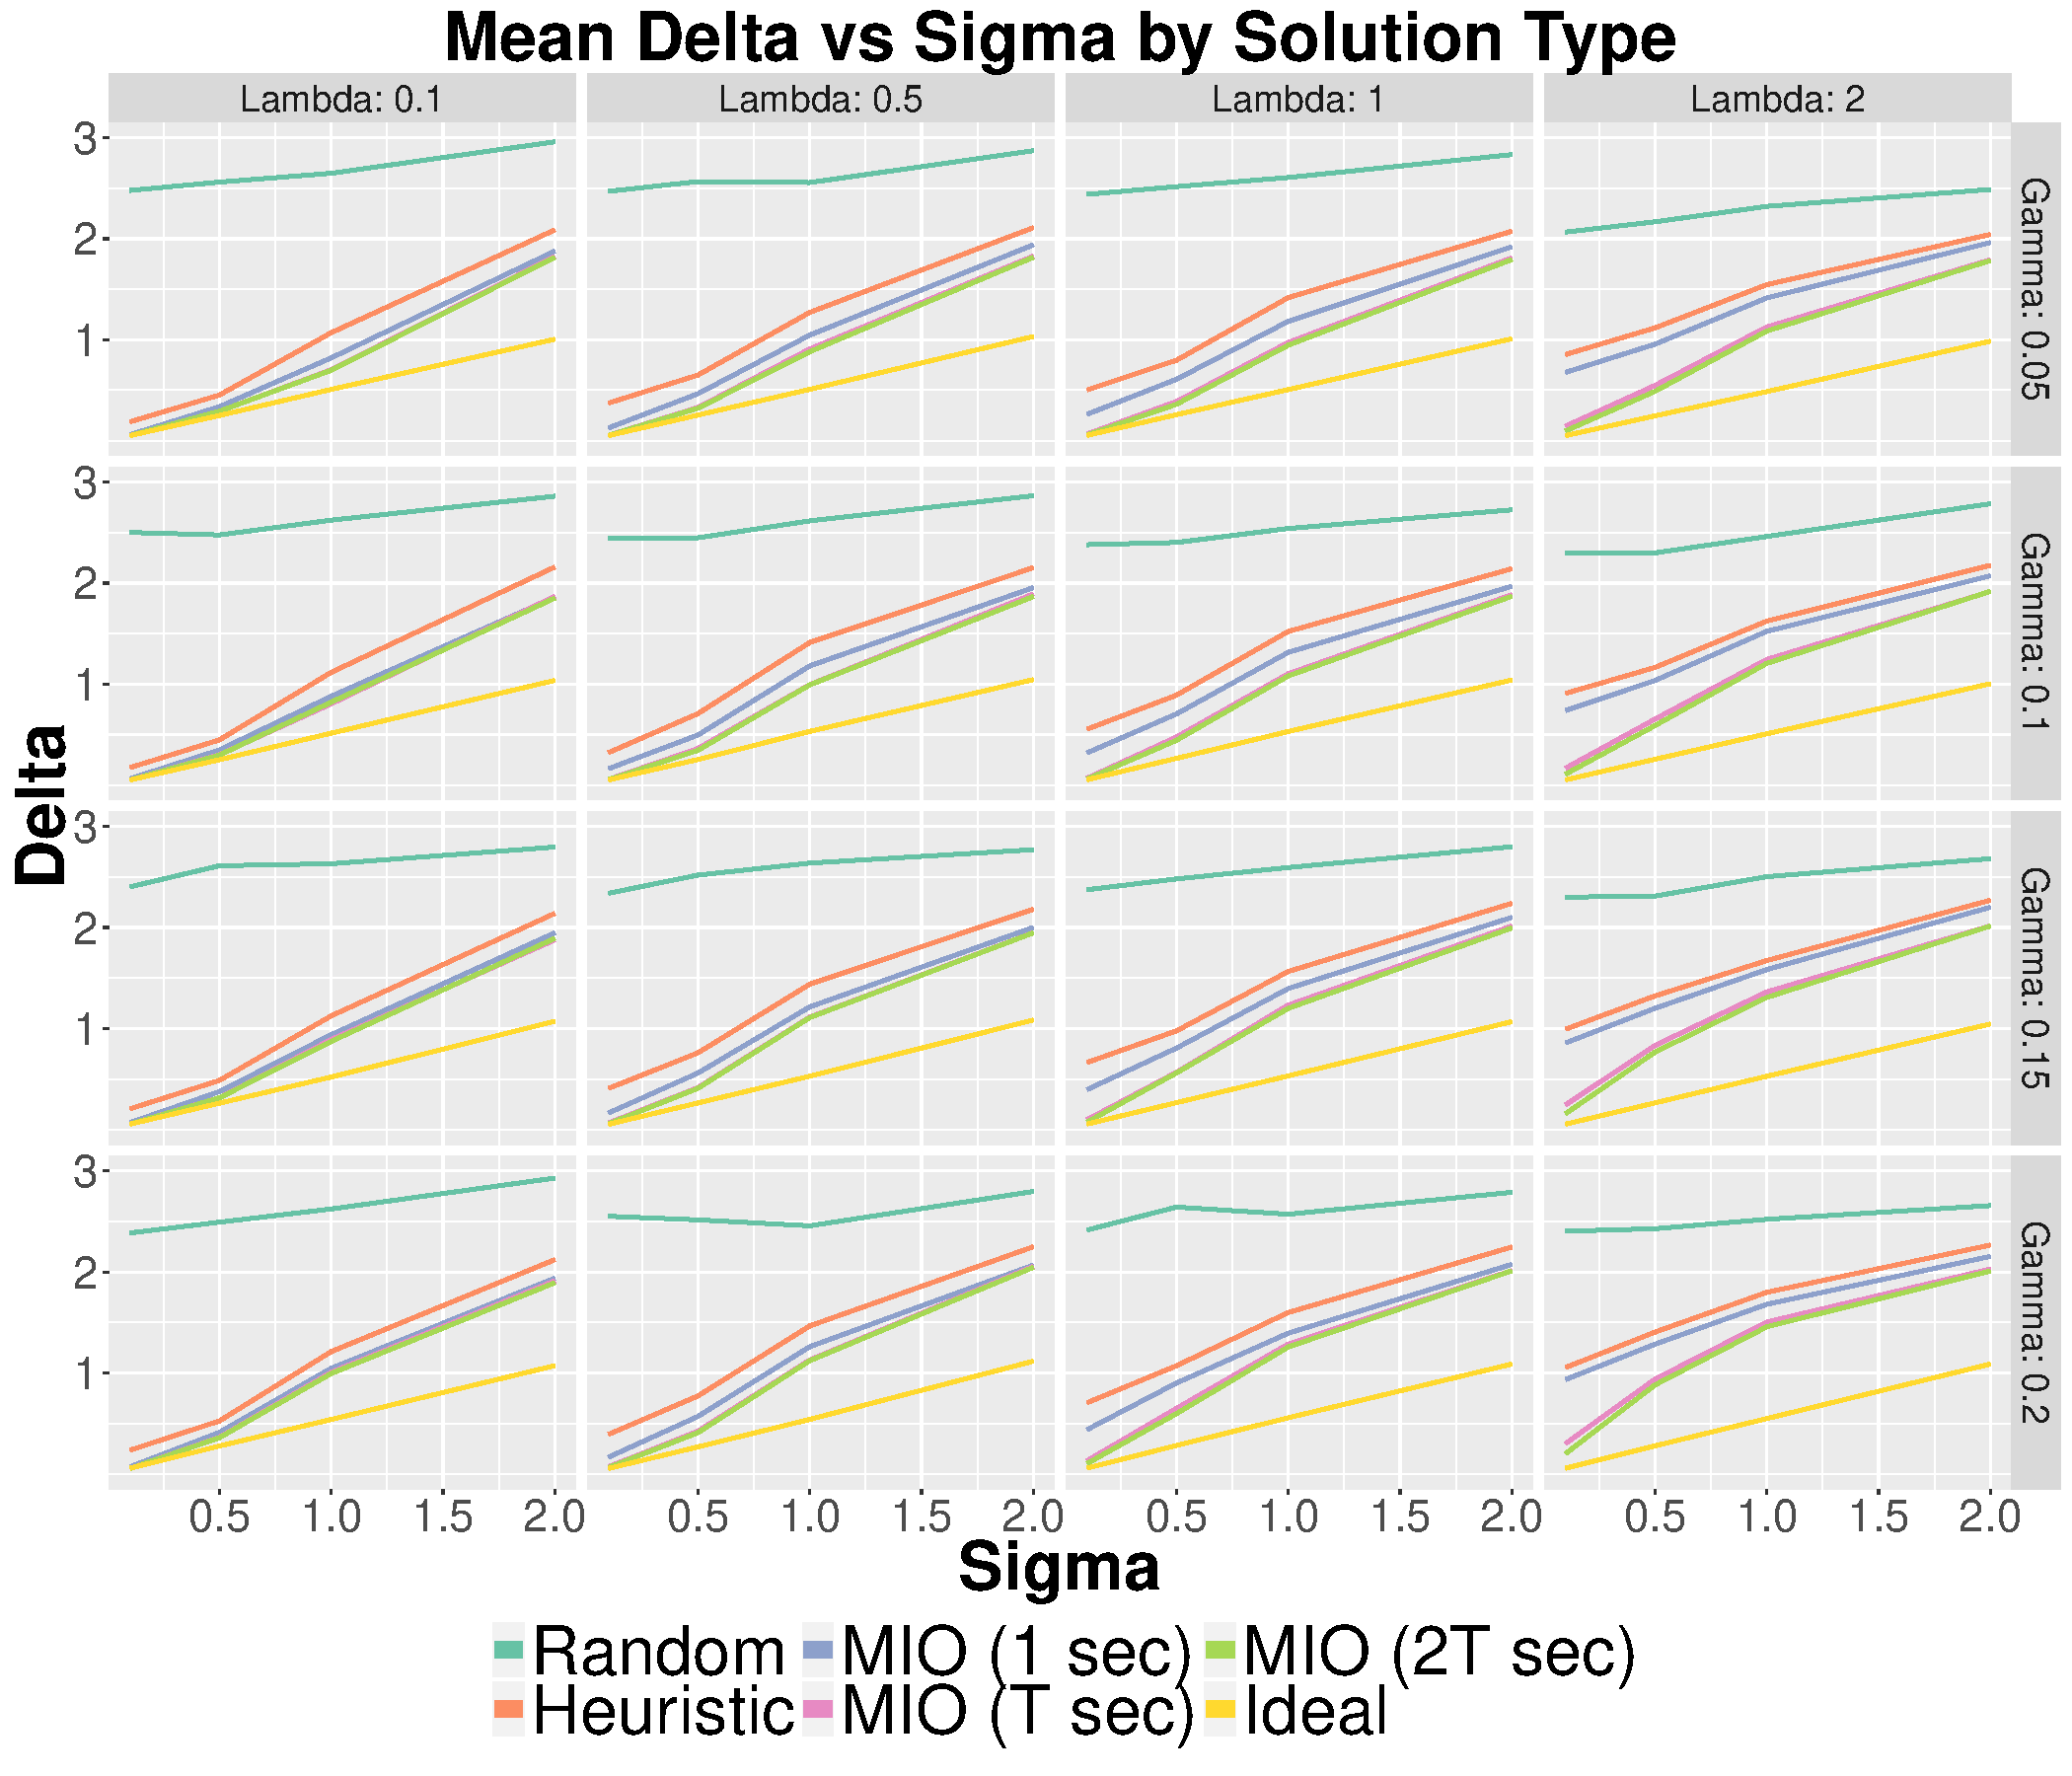
\includegraphics[width=\columnwidth]{../Figures/4_8_Delta}
  \caption{$\delta$ of robust heuristic and MIO as compared to random solutions for scenarios of 4 targets and 8 scans.}
  \label{fig:Robust_4_8_Delta}
\end{figure}

\begin{figure}[ht]
  \centering
  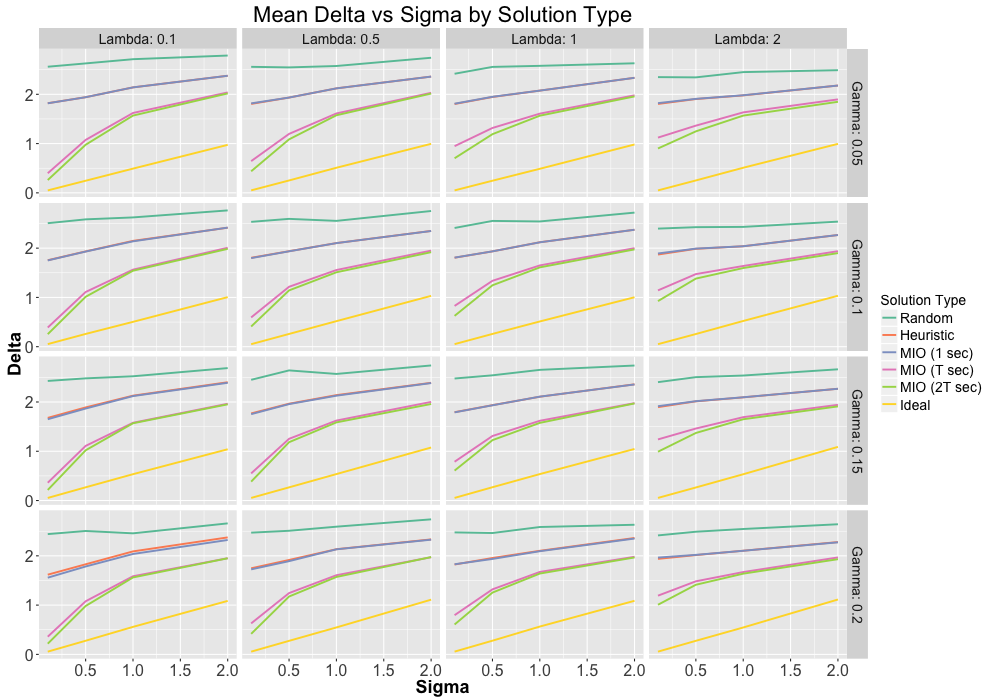
\includegraphics[width=\columnwidth]{../Figures/8_8_Delta}
  \caption{$\delta$ of robust heuristic and MIO as compared to random solutions for scenarios of 8 targets and 8 scans.}
  \label{fig:Robust_8_8_Delta}
\end{figure}

Again, we measure against the basic approaches by comparing Figure~\ref{fig:Robust_4_8_Delta} with the 4 target and 8 scan element of Figure~\ref{Fig:Basic_Delta_Summary}. We see that the robust approaches do not drastically reduce in performance for the easiest robust scenario of $\gamma = 0.05$ and $\lambda = 0.1$. However, the gap in performance between the ideal solution and the solutions of the robust algorithms grows wider with increases in $\sigma$, something that is expected but was not as sizable in the basic experiment. Therefore, the robust approaches may be less robust to increases in $\sigma$ in scenarios with detection ambiguity. However, it also appears that these methods are more robust to increases in the false alarm rate $\lambda$ when it comes to trajectory estimation than they were when it came to data association, especially in the larger scenario shown in Figure~\ref{fig:Robust_8_8_Delta}. We conclude that our robust methods are fairly robust to both increases in the false alarm rate and decreases in trajectory estimation under detection ambiguity, but increasing the signal noise degrades the performance of our methods more so in scenarios with detection ambiguity than in scenarios without detection ambiguity.

\section{Summary and Future Work}\label{sec:Conclusion}
In summary, we presented multi-target tracking approaches which jointly solve the problems of data association and trajectory estimation via global optimization methods using a single objective function. To this end, we proposed the use of a randomized local search heuristic as a warm start for a mixed integer optimization model, and we did so for scenarios with and without detection ambiguity. We accomplish this without the need of a trajectory bank nor the a prior computation of trajectory hypotheses. We showed that the heuristic finds good quality feasible solutions very quickly. We also show that the MIO offers improvement over the heuristic and this improvement is found in real time for applications considered by this paper.  

Furthermore, implementing the heuristic as sliding window algorithm would very likely mitigate this scaling effect in regards to $T$. Rather than solve all scans in a single batch at once, a sliding window algorithm solves a subset of scans, or a smaller window, and advances through all scans sequentially.  As the window progresses forward through the scans,``soft'' decisions are made meaning that the heuristic would begin with the decisions from the previous solution. As scans pass beyond the horizon and out of the sliding window, the decisions become fixed and we refer to them as ``hard" decisions. This process continues until all scans have been processed. The run times of a sliding window variant of the heuristic would not exhibit the curse of dimensionality in $T$ since the number of scans remains constant. Additionally, the heuristic is likely to produce higher quality solutions as a result of these ``soft" decisions of previous steps since it is starting from a solution which is likely to be better than a completely random solution. 

The proposed methods show potential for use in an online algorithm with a sliding window, suggesting one possible area of future work. Additionally, future research could explore the use of more complex penalty functions. One possible idea would be the use of piecewise linear functions which would require further expansion of our formulations. Other areas of future work could seek to relax some of the scenario based assumptions mad in Assumption~\ref{ass:general_assumption}, in particular, extensions to non-linear trajectories or the birth/death of targets. 

\appendices

\section{Detection Ambiguity Penalty Values}\label{app:Penalty_Appendix}
Here we provide recommendations for the tuning of penalty parameters $\theta$ and $\phi$. We begin with an explanation grounded in logic. It can be shown that as the false alarm rate $\lambda$ increases, the number of expected false alarms also increases. Therefore, it stands to reason that as a general rule of thumb the false alarm penalty $\theta$ should decrease as $\lambda$ increases. Similarly, the number of expected missed detections increases as the missed detection probability $\gamma$ increases, and so too the missed detection penalty should decrease. Then it follows logically that the missed detection penalty $\phi$ should increase as $\gamma$ decreases. Furthermore, it is convenient to reason that the value of both of these penalties should somehow be tied to the value of $\sigma$. This is due to the fact that as the noise increases, expect a higher standard deviation for the detections. 
Thus, when assigning false alarms and missed detections, then error will naturally be higher in the objective function. To combat this effect, we should consider increasing both penalties as $\sigma$ increases. Through examination we found these logical concepts to generally hold true across a variety of scenario sizes and difficulties. Using this insight as well as the results of a mini experiment, we tuned our penalties for the robust experiment. The false alarm penalties used are shown in Figure~\ref{tab:Theta_Penalties} and the missed detection penalties are shown in Figure~\ref{tab:Phi_Penalties}.
\begin{table}[ht]
\centering
\begin{tabular}{c|m{1cm}m{1cm}m{1cm}m{1cm}}
  \hline
   & \multicolumn{4}{c}{$\sigma$} \\
   \cline{2-5}
   $\lambda$ & 0.1 & 0.5 & 1.0 & 2.0\\
  \hline
  \hline
   0.1 & 1.7 & 2.6 & 3.1 & 3.5 \\
   0.5 & 1.1 & 1.9 & 2.3 & 2.5 \\ 
   1.0 & 0.9 & 1.2 & 1.6 & 1.8 \\ 
   2.0 & 0.5 & 0.9 & 0.9 & 1.0 \\ 
   \hline
\end{tabular}
\caption{False alarm penalties ($\theta$) as a function of $\lambda$ and $\sigma$.}
\label{tab:Theta_Penalties}
\end{table}
\begin{table}[ht]
\centering
\begin{tabular}{cc|cccc}
  \hline
  & & \multicolumn{4}{c}{$\sigma$} \\
  \cline{3-6}
 $\lambda$ & $\gamma$ & 0.1 & 0.5 & 1 & 2 \\ 
  \hline
  \hline
   0.10 & 0.05 & 0.20 & 0.50 & 0.80 & 0.70 \\ 
   0.10 & 0.10 & 0.10 & 0.30 & 0.50 & 0.50 \\ 
   0.10 & 0.15 & 0.10 & 0.20 & 0.40 & 0.40 \\ 
   0.10 & 0.20 & 0.10 & 0.10 & 0.30 & 0.40 \\ 
   0.50 & 0.05 & 0.20 & 0.50 & 0.80 & 0.80 \\ 
   0.50 & 0.10 & 0.20 & 0.30 & 0.50 & 0.60 \\ 
   0.50 & 0.15 & 0.20 & 0.25 & 0.40 & 0.40 \\ 
   0.50 & 0.20 & 0.10 & 0.20 & 0.30 & 0.40 \\ 
   1.00 & 0.05 & 0.30 & 0.70 & 0.80 & 0.80 \\ 
   1.00 & 0.10 & 0.20 & 0.40 & 0.50 & 0.60 \\ 
   1.00 & 0.15 & 0.20 & 0.25 & 0.40 & 0.40 \\ 
   1.00 & 0.20 & 0.10 & 0.20 & 0.30 & 0.40 \\ 
   2.00 & 0.05 & 0.30 & 0.70 & 0.90 & 1.00 \\ 
   2.00 & 0.10 & 0.20 & 0.50 & 0.60 & 0.60 \\ 
   2.00 & 0.15 & 0.20 & 0.25 & 0.40 & 0.50 \\ 
   2.00 & 0.20 & 0.10 & 0.20 & 0.30 & 0.40 \\ 
   \hline
\end{tabular}
\caption{Missed detection penalties ($\phi$) as a function of $\lambda$, $\gamma$, and $\sigma$.}
\label{tab:Phi_Penalties}
\end{table}

\section{Robust MIO With Number of Targets as a Decision Variable}\label{app:Robust_Appendix}
For completeness here we present an alternative approach to solving the MTT problem with detection ambiguity. This MIO model is an extension to \eqref{eq:simple_robust} that directly determines the number of targets via optimization by incorporating additional variables and constraints into framework of the formulation. 

\subsection{Decision Variables}
Because we do not assume a fixed number of targets, this decision must now be made by the model. Toward this goal, we introduce a new binary decision variable $w_{j}$ to indicate whether or not trajectory \textit{j} corresponds to an existing target. Any detections assigned to a non-existing target would be a false alarm. 
\[w_{j} = 
\begin{cases}
1, & \text{if trajectory \textit{j} exists,}\\
0, & \text{otherwise.}
\end{cases}\]

\subsection{Constraints}
Most constraints remain similar to their original counterparts in \eqref{eq:simple_robust}, except for slight adjustments needed to account for the possibility that some trajectories may not exist. Explicitly, the number of possible trajectories is now $N_{1}$ so all instances of summing over \textit{j} must be changed accordingly. For example, we adjust \eqref{eqn: FA Simple} and \eqref{eqn: MD Total} as follows: 
\begin{align*}
\sum_{j=1}^{N_{1}} y_{itj} + F_{it} = 1 \qquad \forall i,t,\\
\sum_{j=1}^{N_{1}} \sum_{t=1}^{T} M_{jt} = TM.
\end{align*}

By the same accord \eqref{eq: } no longer equates to 1 because some trajectories may not exist. Therefore we say all \textit{existing} trajectories must either be assigned a detection or a missed detection,
\begin{align}\label{eqn: Existing Targets}
\sum_{i=1}^{n_{t}} y_{itj} + M_{jt} = w_{j} \qquad \forall j,t.
\end{align}

Moreover, we restrict $\alpha_{j}$ and $\beta_{j}$ to be zero if trajectory \textit{j} does not exist. This ensures only existing trajectories are penalized in the objective function. 
\begin{align*}
|\alpha_{j}|+|\beta_{j}| \leq M_{0}w_{j}\qquad \forall j.
\end{align*}

We can actually reduce the symmetry that is inherent to this formulation. Since $N_{0} \leq P \leq N_{1}$, we can set $w_j=1$ for all $j=1,\ldots,N_0$, which leaves us with only $N_1-N_0$ additional binary variables. We simply need the additional constraint
\begin{align*}
w_{N_0+1}\geq ...\geq w_{N_1},
\end{align*}
which reduces the symmetry of the formulation, and thus making it efficiently solvable. 

\subsection{MIO with Number of Targets as a Decision Variable}
Incorporating these additional variables and constraints, we arrive at the following complete alternative formulation.
\begin{align*}
\underset{\psi_{jt}}{\text{minimize: }} & \sum_{j=1}^{N_{1}} \sum_{t=1}^{T} \psi_{jt} + \theta \cdot TF + \phi \cdot TM\\
\text{subject to: }	& \sum_{j=1}^{N_{1}} y_{itj} + F_{it} = 1 \qquad \forall i,t \nonumber\\
				& \sum_{i=1}^{n_{t}} y_{itj} + M_{jt} = 1 \qquad \forall j=1,...,N_{0},t \nonumber \\
				& \sum_{i=1}^{n_{t}} y_{itj} + M_{jt} = w_{j} \qquad \forall j=N_{0},...,N_{1},t \nonumber \\
				& \sum_{i=1}^{n_{t}} \sum_{t=1}^{T} F_{it} = TF \nonumber \\
				& \sum_{j=1}^{N_{1}} \sum_{t=1}^{T} M_{jt} = TM \nonumber \\
				& w_{N_0+1}\geq ...\geq w_{N_1} \nonumber \\
				& |\alpha_{j}|+|\beta_{j}| \leq M_{0}w_{j}\qquad \forall j \nonumber \\
				& x_{it}y_{itj} + M_{t}(1-y_{itj}) \geq z_{jt} \qquad \forall i,t,j \nonumber \\
				& x_{it}y_{itj} - M_{t}(1-y_{itj}) \leq z_{jt} \qquad \forall i,t,j \nonumber \\
				& z_{jt} - \alpha_{j} - \beta_{j}t \leq \psi_{jt} \qquad \forall j,t \nonumber \\
				& -(z_{jt} - \alpha_{j} - \beta_{j}t) \leq \psi_{jt} \qquad \forall j,t \nonumber \\
			 	& y_{itj} \in \{0,1\} \quad \forall i,t,j \nonumber \\
				& \alpha_{j} \in \mathbb{R}^n,\quad \beta_{j} \in \mathbb{R}^n,\quad w_{j} \in \mathbb{R}^n \quad \forall j \nonumber \\
				& z_{jt} \in \mathbb{R}^n, \quad \forall j,t. \nonumber
\end{align*}

\subsection{Extension of Robust Heuristic}
Insert brief discussion about how this heuristic would be identical to the one proposed previously, except a number of estimated targets would be randomly selected during the initialization process and then the heuristic would progress identically to the robust heuristic already proposed.

\section{Trajectory Assignment Pairing}\label{app:Assignment_Appendix}
In order to analyze the performance of a multi-target tracking algorithm, we must find the best matching of the true trajectories of the scenario and the estimated trajectories of the algorithm solution. Put differently, we wish to find a set of assignment pairings which match true and estimated trajectories. Here we present a linear optimization model which solves for the globally optimal assignment pairings of true and estimated trajectories. In addition, we discuss the required 

The goal of this assignment problem is to optimally assign pairs of true trajectories \textit{i} to estimated trajectories \textit{j} if there exists such a pairing to be made. Only a single set of decision variables are needed to determine if the true trajectory \textit{i} should be assigned to the estimated trajectory \textit{j} or not. 
\[y_{ij} = 
\begin{cases}
1, & \text{if true trajectory \textit{i} is assigned}\\
    & \text{ to estimated trajectory \textit{j},}\\
0, & \text{otherwise.}
\end{cases}\]

Remember that we denote the true position of trajectory \textit{i} at scan \textit{t} with $\bar{x}_{it}$ and the estimated position of trajectory \textit{j} at scan \textit{t} with $\hat{x}_{jt}$. Then the cost $c_{ij}$ of assigning true trajectory \textit{i} to estimated trajectory \textit{j} is the norm distance between these two trajectories as measured at each scan. 
\begin{align*}
	c_{ij} = \sum_{t=1}^{T} \|\bar{x}_{it} - \hat{x}_{jt}\|
\end{align*}
If we denote the true number of targets as $P_{\text{true}}$ and the estimated number of targets as $P_{\text{estimated}}$ then the objective of the integer optimization model would be:
\begin{align*}
\underset{y_{ij}}{\text{minimize: }} & \sum_{i=1}^{P_{\text{true}}} \sum_{j=1}^{P_{\text{estimated}}} c_{ij}y_{ij}
\end{align*}

When the number of true targets is equal to the number of estimated targets ($P_{\text{true}} = P_{\text{estimated}} = P$), we simply require two equality constraints to ensure that each true trajectory \textit{i} is assigned to exactly one estimated trajectory \textit{j} and vice versa. 
\begin{align}\label{eqn:assignment_1}
\sum_{i=1}^{P} y_{ij} = 1 \qquad \forall j = 1,...,P
\end{align}
\begin{align}\label{eqn:assignment_2}
\sum_{j=1}^{P} y_{ij} = 1 \qquad \forall i = 1,...,P
\end{align}

However, when the number of estimated trajectories differs from the number of true trajectories, these constraints must be modified slightly. In the case where the number of true targets exceeds the estimated number of targets ($P_{\text{true}}\geq P_{\text{estimated}}$), we restrict each true trajectory \textit{i} to the assignment of \textit{at most} one estimated trajectory \textit{j}, and Equation~\ref{eqn:assignment_1} is modified to:
\begin{align*}
\sum_{i=1}^{P_{\text{true}}} y_{ij} \leq 1 \qquad \forall  j = 1,...,P_{\text{estimated}}.
\end{align*}

On the contrary, when the number of estimated targets exceeds the true number of targets ($P_{\text{true}}\leq P_{\text{estimated}}$), then we restrict each estimated trajectory \textit{j} to the assignment of \textit{at most} one true trajectory \textit{i}, and Equation~\ref{eqn:assignment_2} is modified to:
\begin{align*}
\sum_{j=1}^{P_{\text{estimated}}} y_{ij} \leq 1 \qquad \forall i = 1,...,P_{\text{true}}.
\end{align*}

In summary, the generalized integer optimization assignment model is presented below.  
\begin{align*}
\underset{y_{ij}}{\text{minimize: }} & \sum_{i=1}^{P_{\text{true}}} \sum_{j=1}^{P_{\text{estimated}}} c_{ij}y_{ij}\\
\text{subject to: }	& \sum_{i=1}^{P_{\text{true}}} y_{ij} = 1 \qquad \forall j = 1,...,P_{\text{estimated}} \nonumber \\
				& \sum_{j=1}^{P_{\text{estimated}}} y_{ij} = 1 \qquad \forall i = 1,...,P_{\text{true}} \nonumber \\
				& y_{ij} \in \{0,1\} \quad \forall i = 1,...,P_{\text{true}},j = 1,...,P_{\text{estimated}} \nonumber
\end{align*}
This model is vital to scoring the performance of an MTT algorithm's solution because it ensures the globally optimal pairing of true and estimated trajectories.




\section*{Acknowledgments}
The authors would like to thank Sung-Hyun Son, Ph.D. and Steven Relyea at Lincoln Laboratories for introducing us to the MTT problem and for their ongoing guidance throughout this work. Additionally, we would like to thank Lincoln Laboratories and the LLGrid team for their continual support in running our experiments. 

This material is based upon work supported by the Air Force under Air Force Contract No. FA8721-05-C-0002 and/or FA8702-15-D-0001. The views expressed in this document are those of the authors and do not reflect the official policy or position of the United States Air Force, the United States Department of Defense or the United States Government.

%\IEEEtriggeratref{15}
% The "triggered" command can be changed if desired:
%\IEEEtriggercmd{\enlargethispage{-5in}}


\bibliographystyle{IEEEtran}
\bibliography{Bibliography}

\end{document}